\documentclass{beamer}
\usepackage{color}
\usepackage{graphicx}
\usepackage[T1]{fontenc}
\usepackage[utf8]{inputenc}
\usepackage[english]{babel}
\usepackage{amsfonts,amsmath,amssymb,amsthm}
\usepackage{alltt}
\usepackage{mathrsfs} 
\usepackage{multicol}
\usepackage{subfigure}
\usepackage{ragged2e}
\usepackage{booktabs}
\usepackage{makecell}
\usepackage{multirow}

\usefonttheme{professionalfonts}

\usetheme{cinvestavbokumantle}
\title{High Quality Labeling}
\author{Andrea Elizabeth González Ramírez}

\begin{document}

\begin{frame}
    \titlepage
    \thispagestyle{empty}
\end{frame}

\section{}
\begin{frame}
    \begin{figure}
        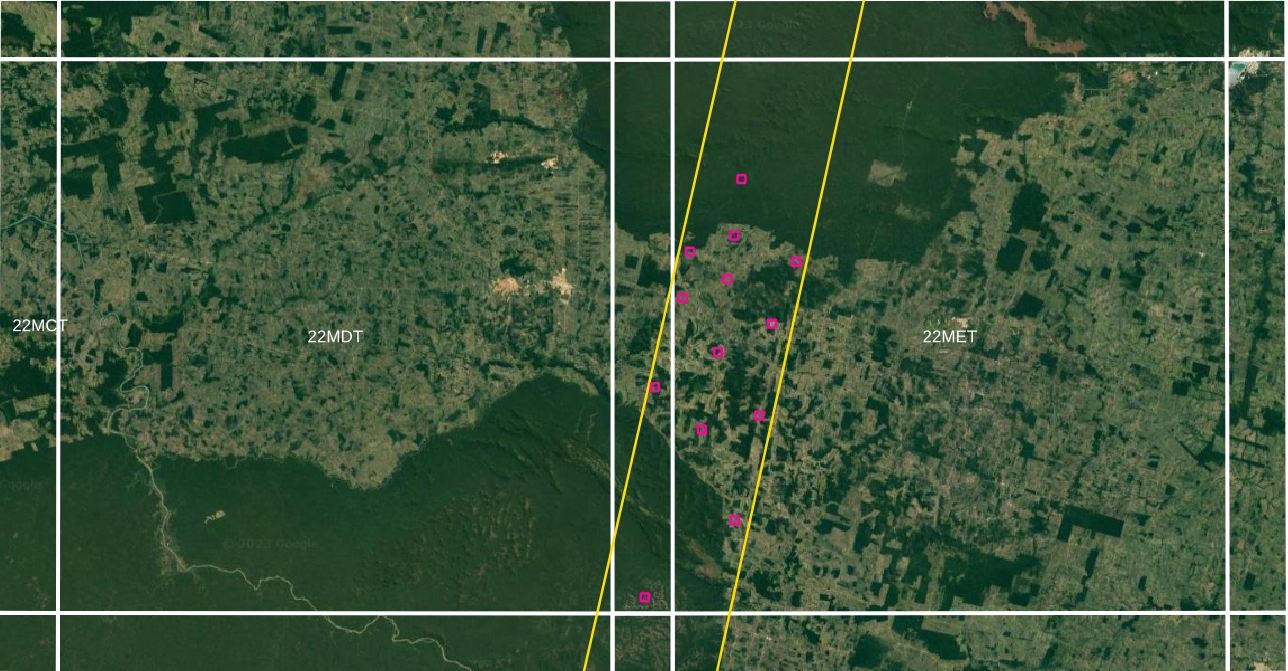
\includegraphics[width=10cm]{Figures/v3/main/overlaping_polygons_1.png}
        \caption{All polygons over area of interest: 22MET overlap.}  
        \centering
    \end{figure}
\end{frame}

\begin{frame}{Updates}
    \begin{itemize}
        \item Computed the Brightness Index
        \item Computed the error with Euclidean distance
    \end{itemize}
\end{frame}

\section{Dataset}
\begin{frame}{Dataset}
    \begin{minipage}{0.65\textwidth}
        \begin{table}
            \scriptsize
            \begin{tabular}{c|c}
                \hline
                \multicolumn{2}{c}{\textbf{Dataset}} \\
                \hline  	
                Tiles &  22MET \\
                Number of polygons & 12 \\
                Time range & \makecell{2021-05-01 \\ 2021-09-30} \\
                Total number observations & 61\\
                Number with HQ observations & 34 \\
                Number of spectral bands & 12*\\
                Number of features & 13 (bands + ndvi)\\
                \hline
                \multicolumn{2}{c}{*All spectral bands except B10} \\
            \end{tabular}
            \caption{Description of the dataset.}
        \end{table}
    \end{minipage}
    \begin{minipage}{0.3\textwidth}
        \begin{table}
            \scriptsize
            \begin{tabular}{c|c}
            \hline
                \multicolumn{2}{c}{\textbf{Classes}} \\ \hline
                Fully Cloudy & FC \\
                Partly Cloudy& PC \\
                Full Shadow & FS \\
                Partly Shadow& PS \\
                Low quality & LQ \\
                Medium quality & MQ\\
                High quality & HQ \\
                \hline
            \end{tabular}
            \caption{Description of labels.}
        \end{table}
    \end{minipage}
\end{frame}

\begin{frame}{Brightness Index (BI)}
    \begin{equation}
        BI = \sqrt{\frac{ (B4^2 + B3^2 + B2^2)}{3}}
    \end{equation}
    
\end{frame}

\section{Labeling}
\begin{frame}
    \begin{figure}
        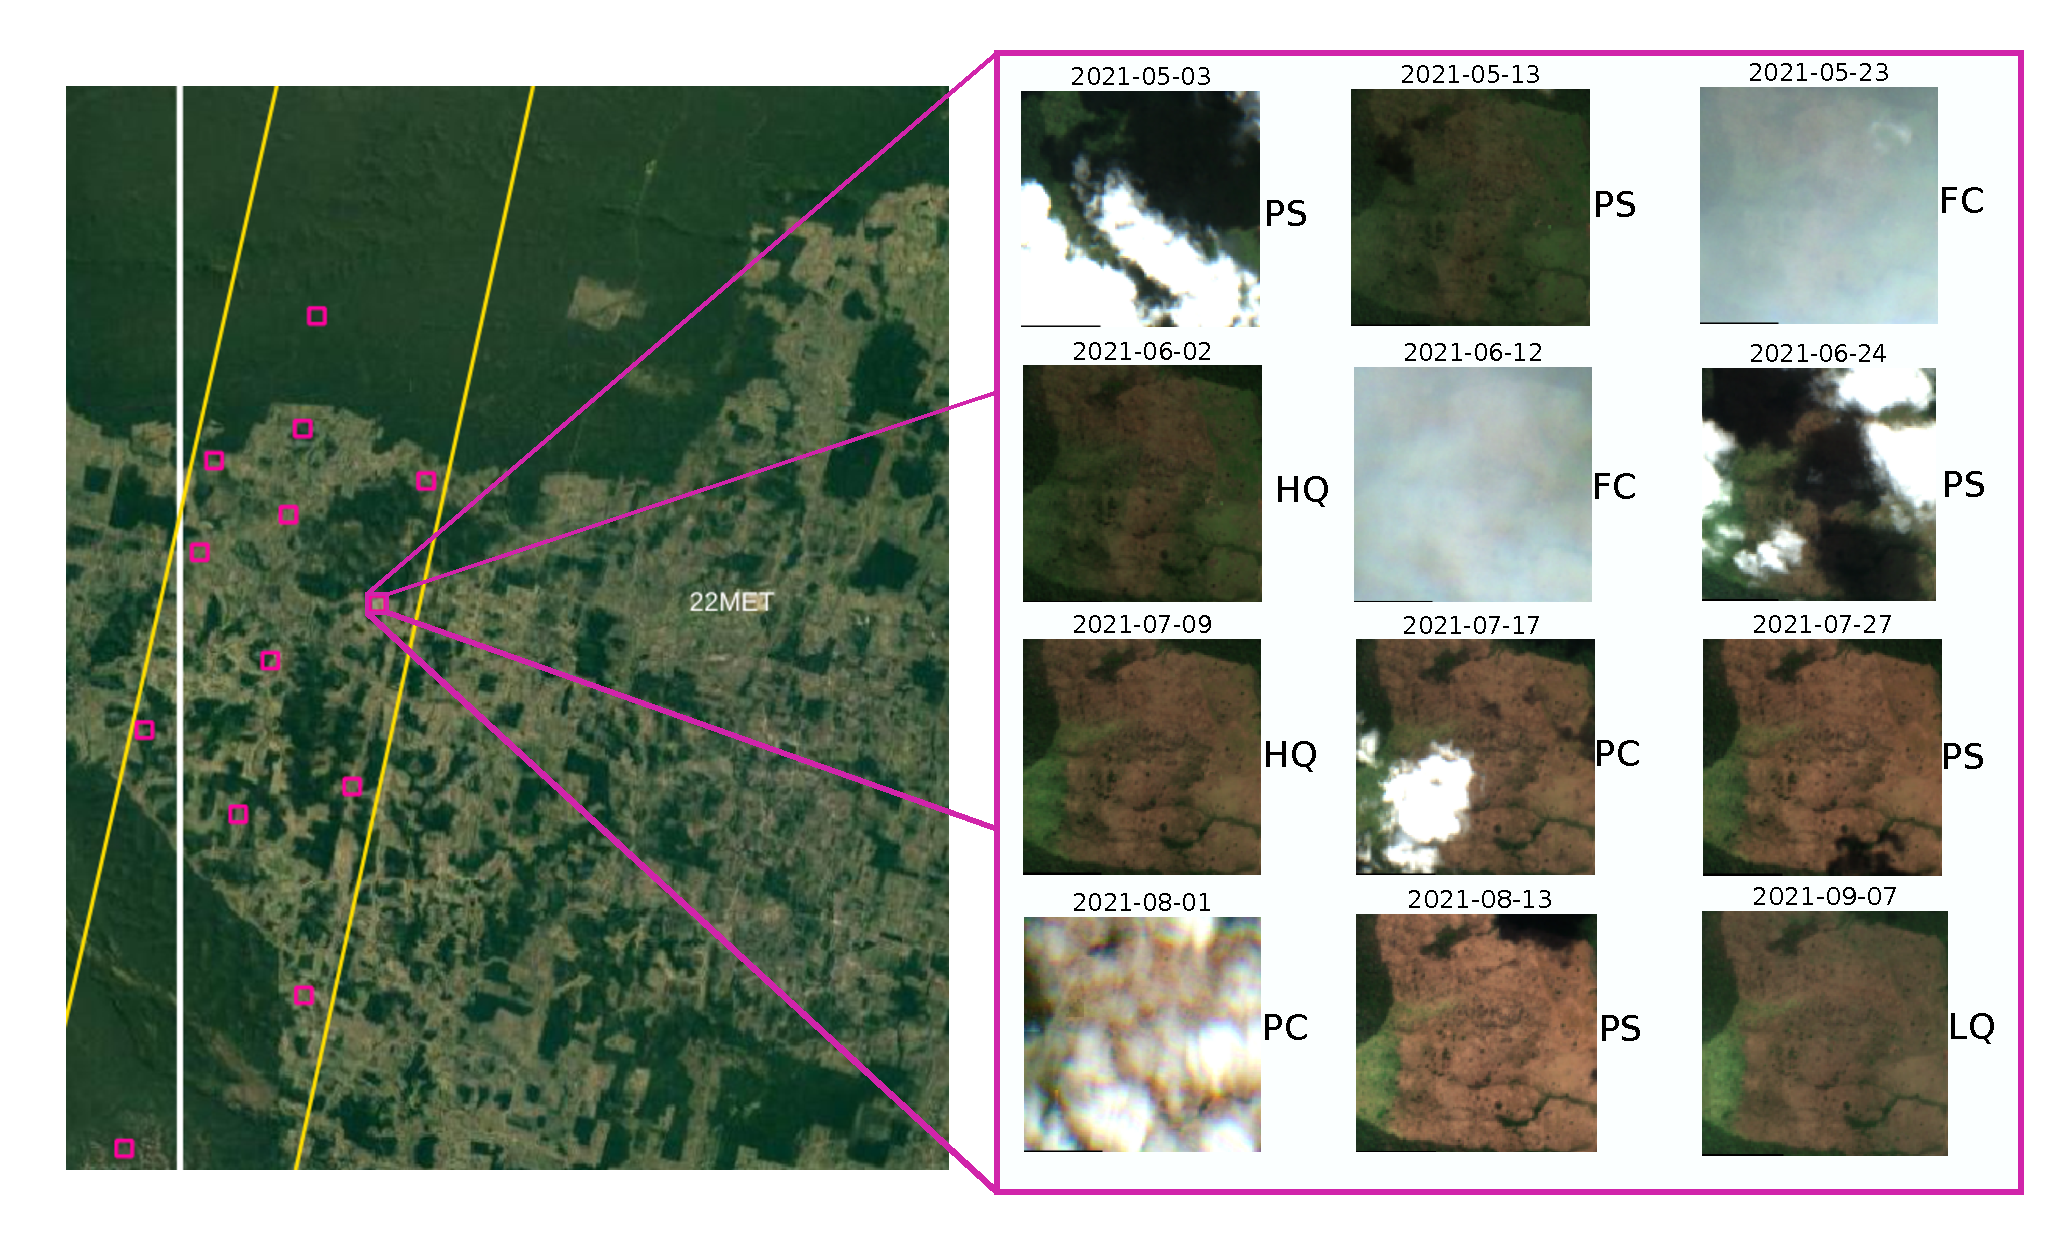
\includegraphics[width=10cm]{Figures/v3/labeling/polygon_0.pdf}
        \caption{Polygon 1. Examples of some observation/labels.}  
        \centering
    \end{figure}
\end{frame}

\begin{frame}
    \begin{figure}
        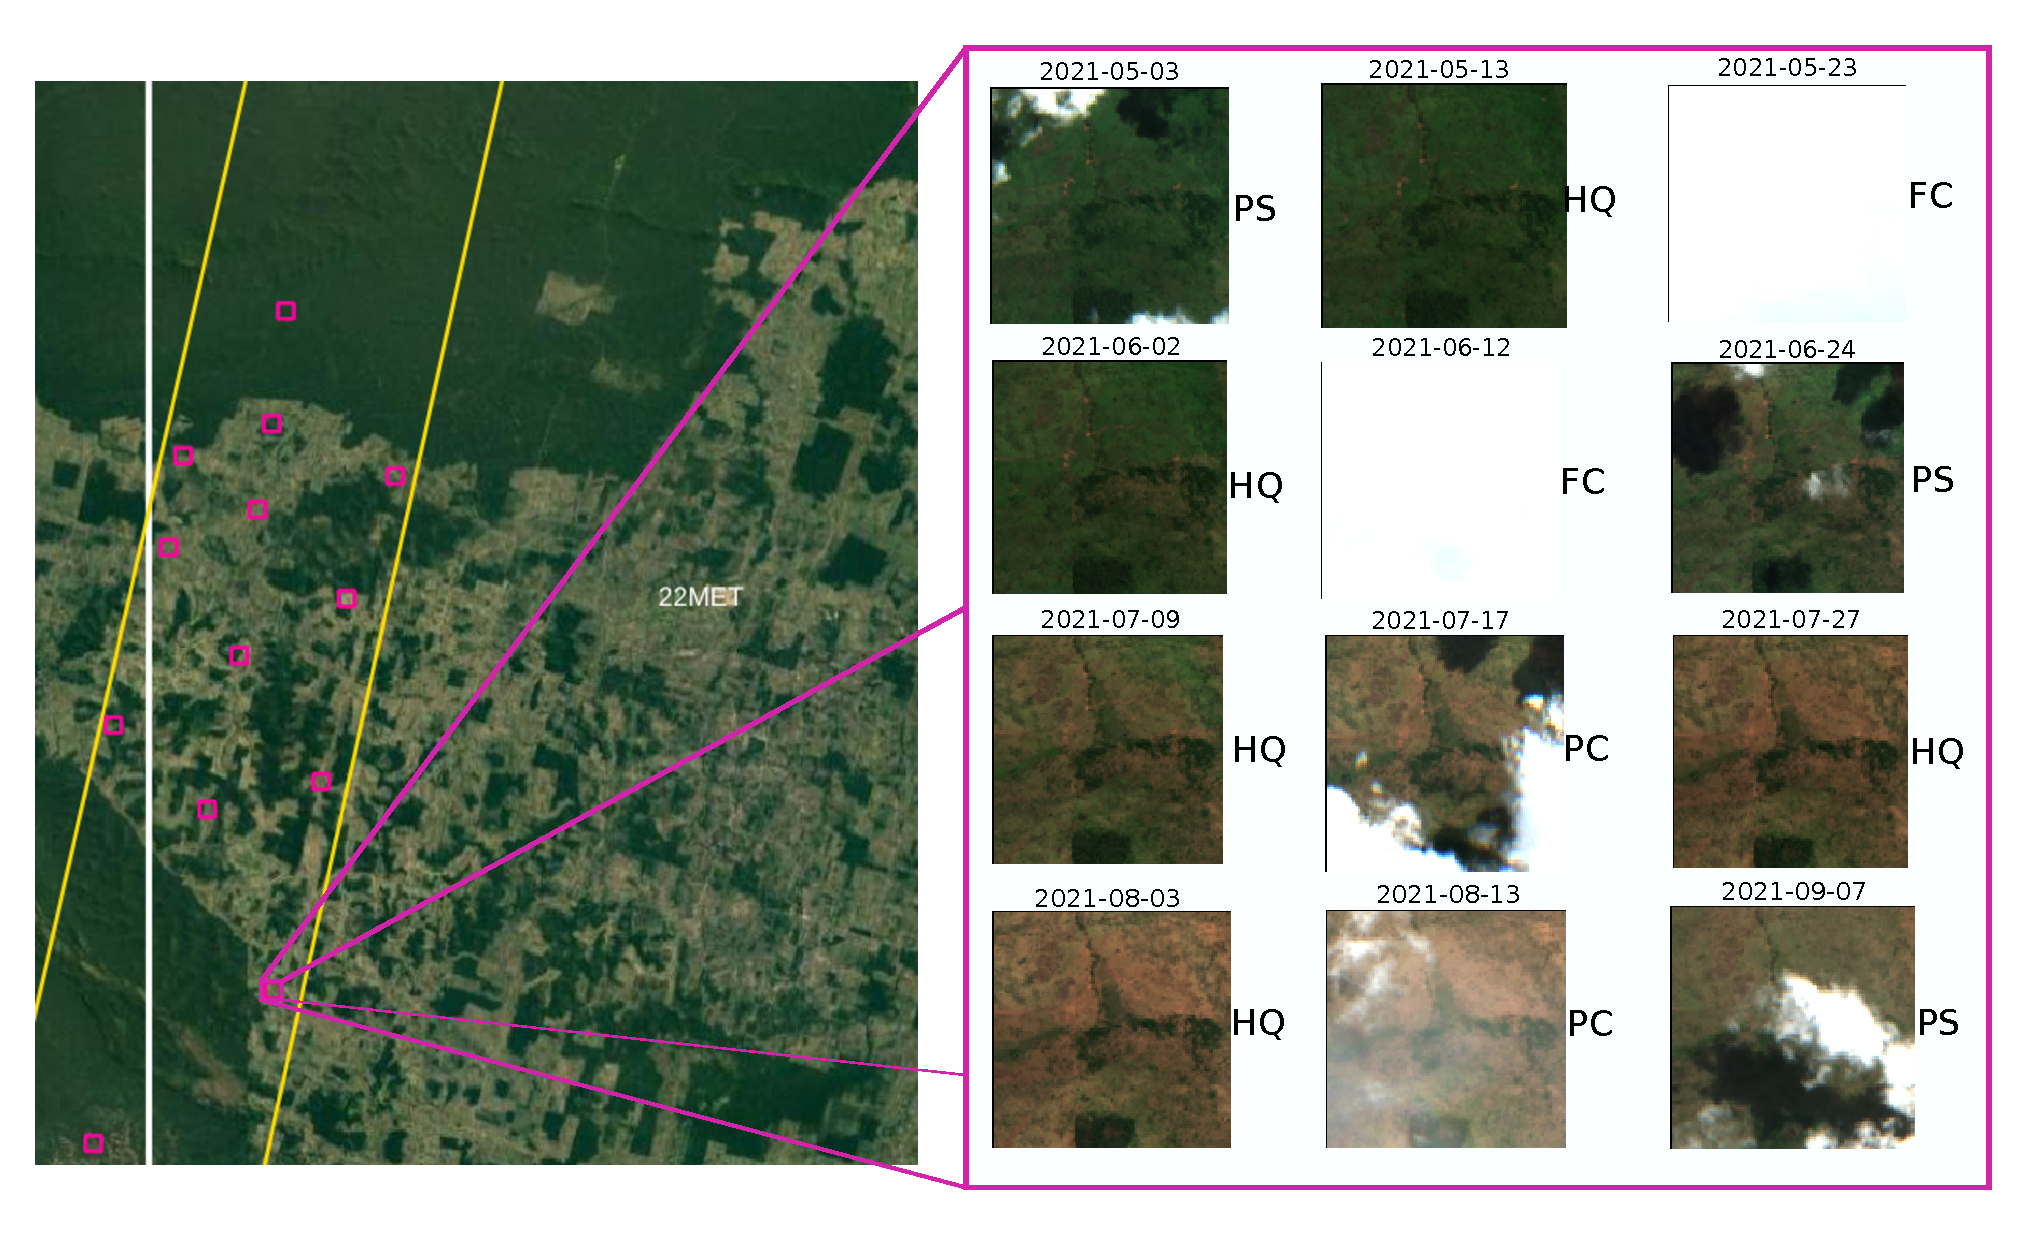
\includegraphics[width=10cm]{Figures/v3/labeling/polygon_2.pdf}
        \caption{Polygon 2. Examples of some observation/labels.}  
        \centering
    \end{figure}
\end{frame}

\begin{frame}
    \begin{figure}
        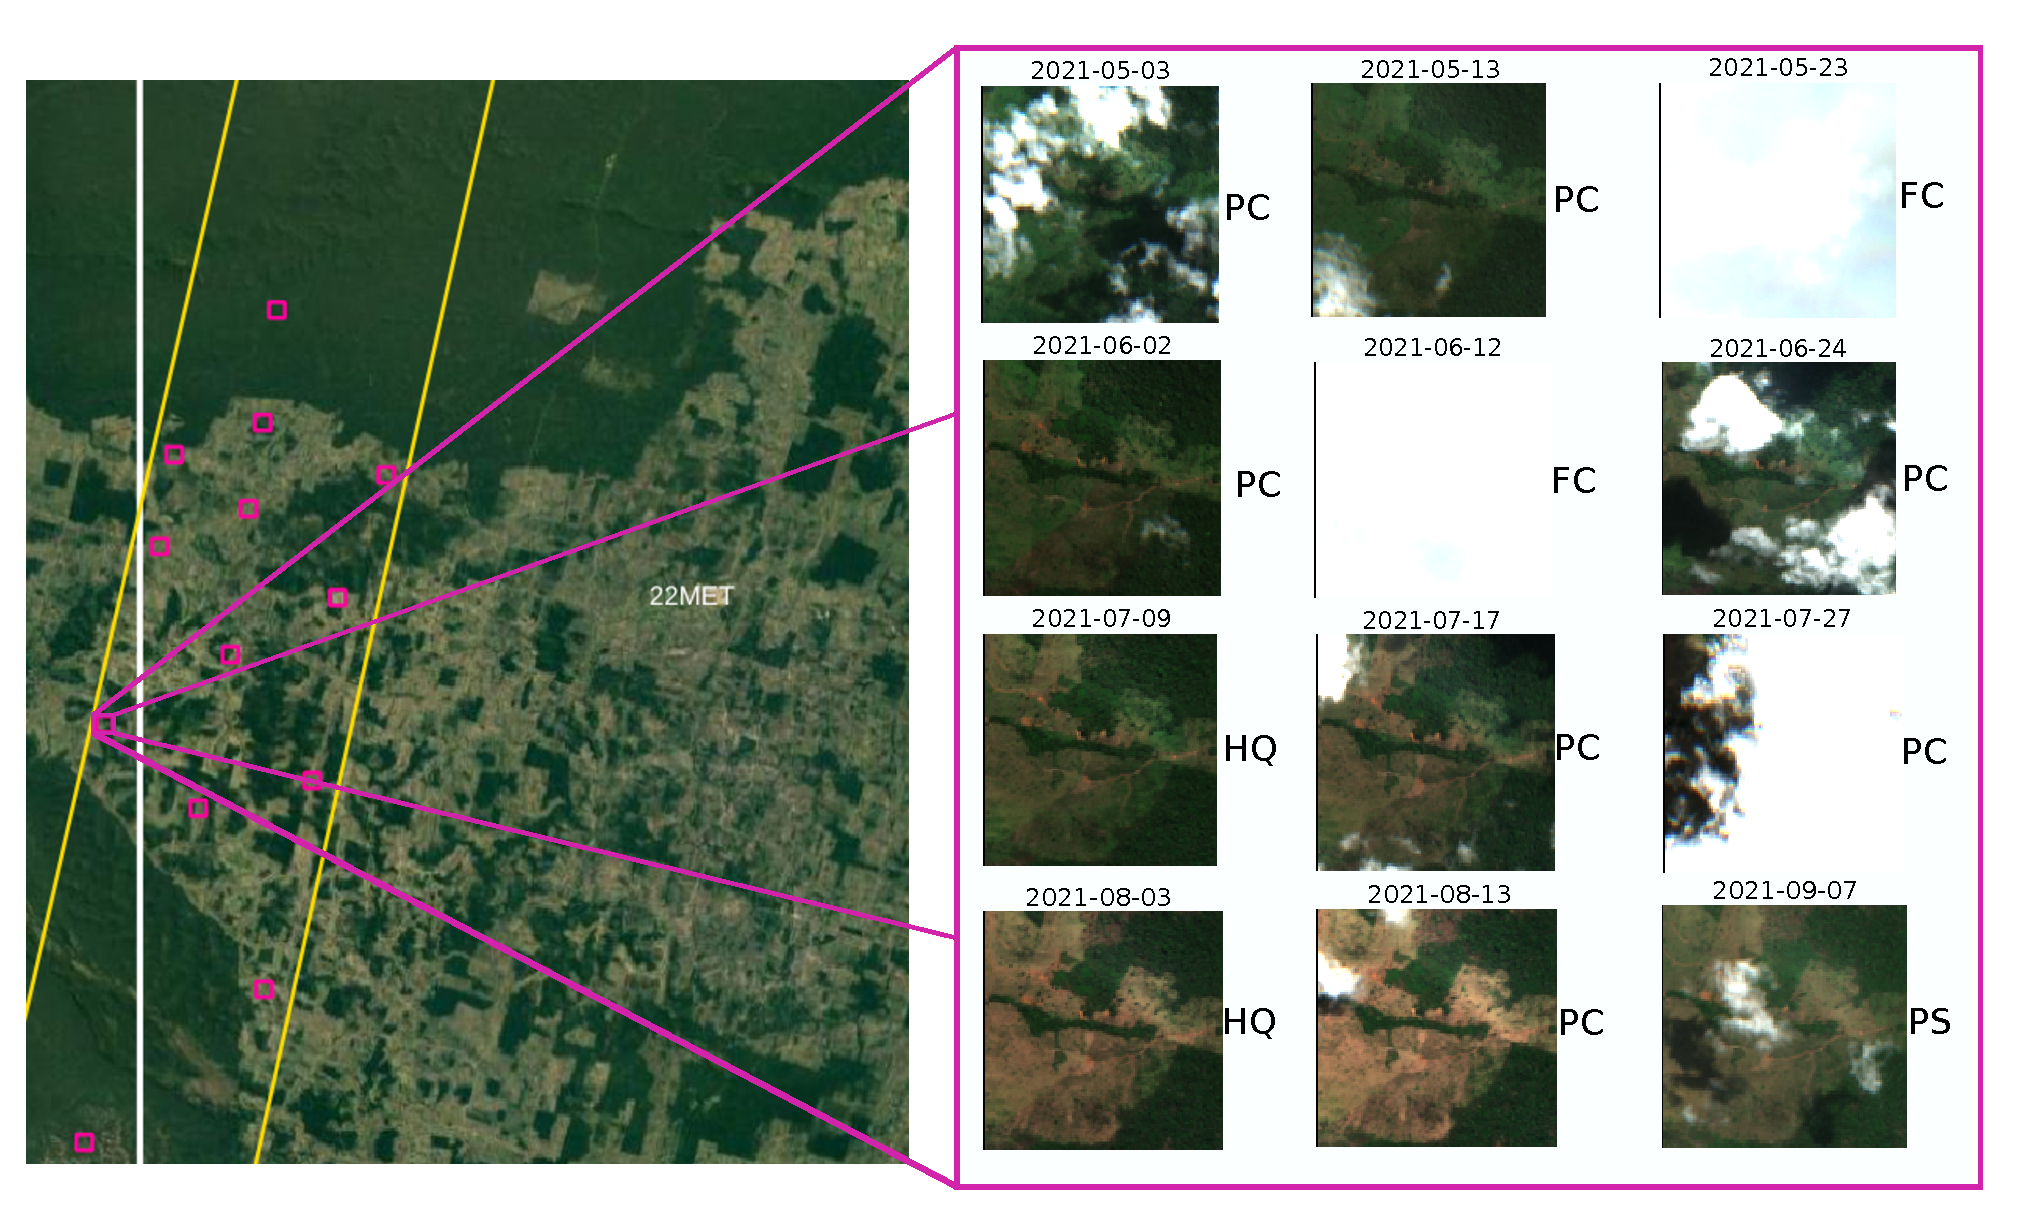
\includegraphics[width=10cm]{Figures/v3/labeling/polygon_4.pdf}
        \caption{Polygon 3. Examples of some observation/labels.}  
        \centering
    \end{figure}
\end{frame}

\begin{frame}
    \begin{figure}
        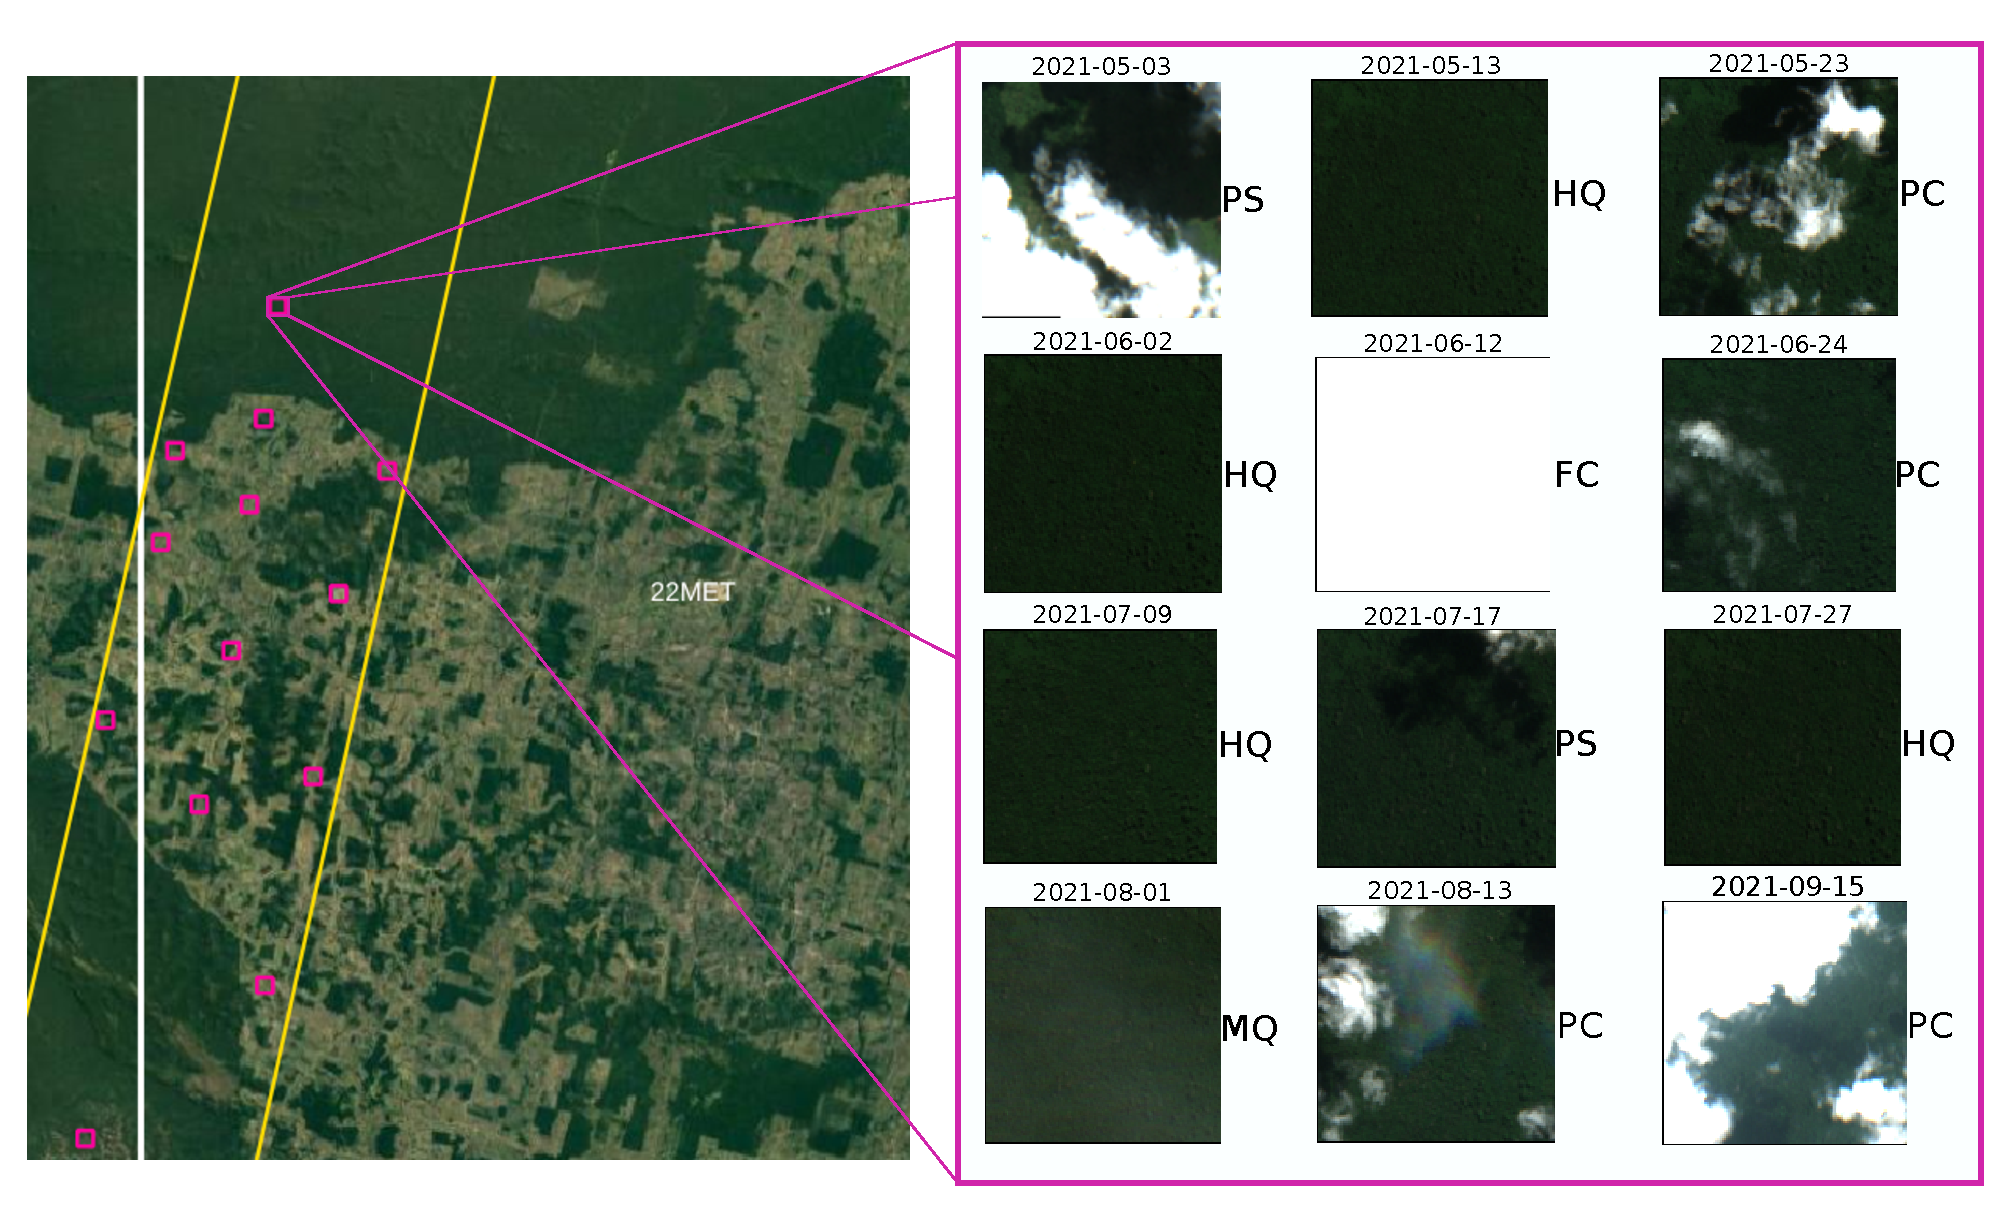
\includegraphics[width=10cm]{Figures/v3/labeling/polygon_11.pdf}
        \caption{Polygon 4. Examples of some observation/labels.}  
        \centering
    \end{figure}
\end{frame}

\section{Training}
\begin{frame}{Implementation details of the AE}
    \begin{minipage}{0.6\textwidth}
        \begin{figure}
            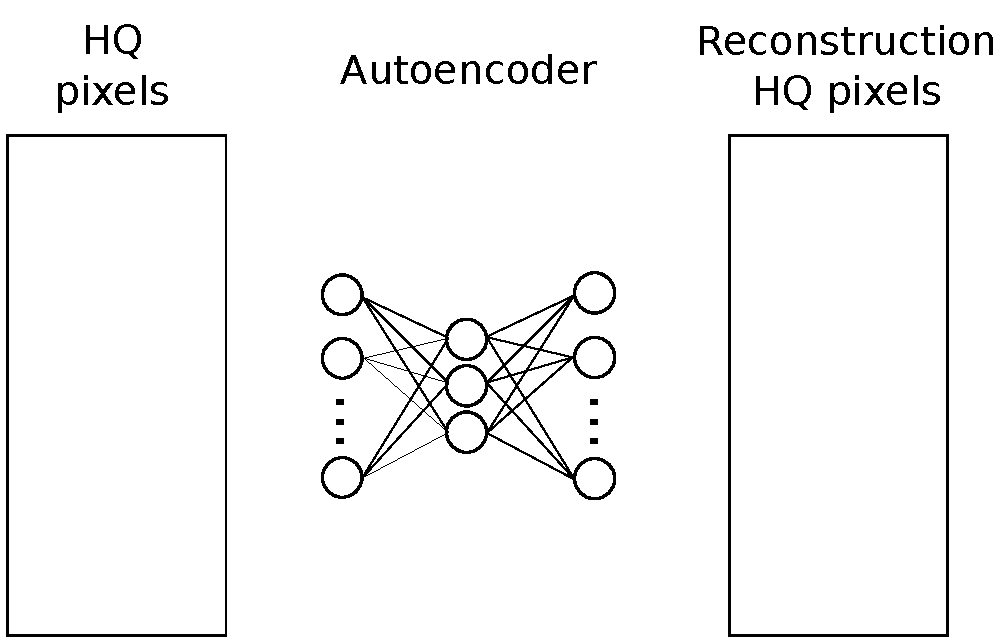
\includegraphics[width=0.6\textwidth]{Figures/v3/main/training.pdf}
            \caption{Workflow of training.}  
        \end{figure}
        \begin{figure}
            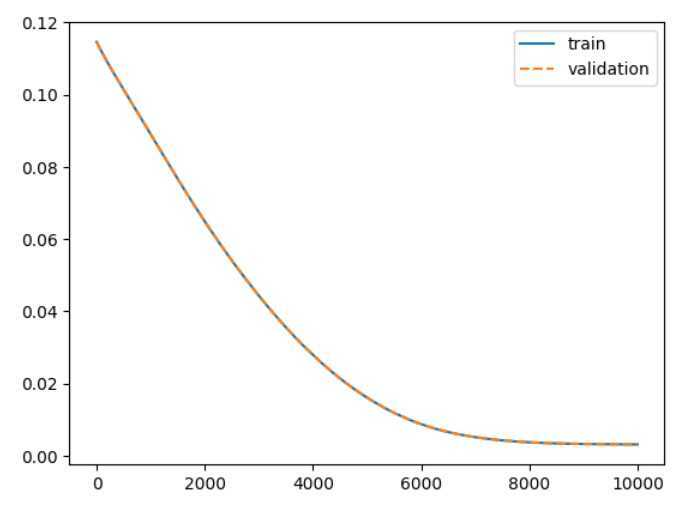
\includegraphics[width=0.55\textwidth]{Figures/v3/main/loss.jpg}
            \caption{Loss function.}  
            \centering
        \end{figure}
    \end{minipage}
    \begin{minipage}{0.35\textwidth}
        \begin{table}
            \scriptsize
            \begin{tabular}{c|c}
            \hline
                \multicolumn{2}{c}{Hyperparameters} \\ \hline
                Training size & 90$\%$ \\ [1ex]
                Validation size & 10$\%$ \\ [1ex]
                Epochs & 10000 \\ 
                Batch size & 0.1 \\ 
                Units in hidden layers & 3 \\ 
                Learning rate & 1e-5 \\ 
                Optimizer & Adam \\ 
                Loss & MSE \\ \hline
            \end{tabular}
            \caption{Setting up of the Autoencoders hyperparameters.}
        \end{table}
    \end{minipage}
\end{frame}

\section{Results}
% \begin{frame}{Date: 2021-05-13}
% \centering
%     \begin{tabular}{cc}
%     TCI & Error map\\
%     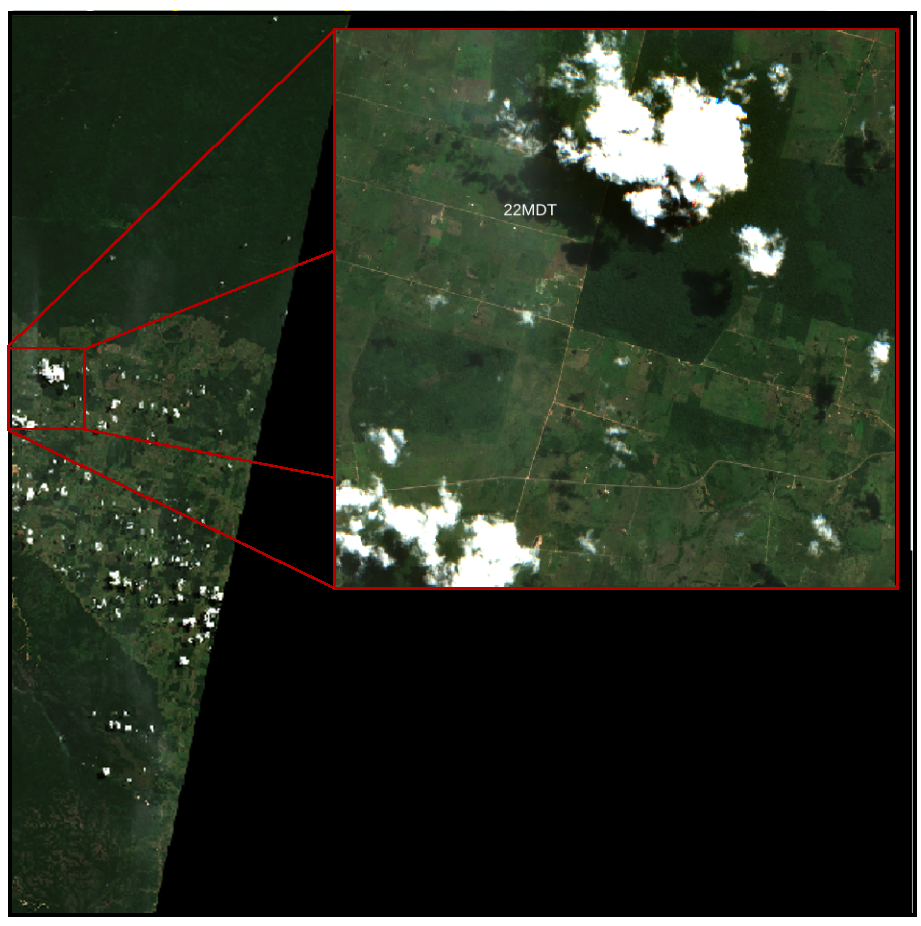
\includegraphics[width=2.5cm]{Figures/v3/20210513/111-TCI_with_zoom_roi.pdf}
%     &
%     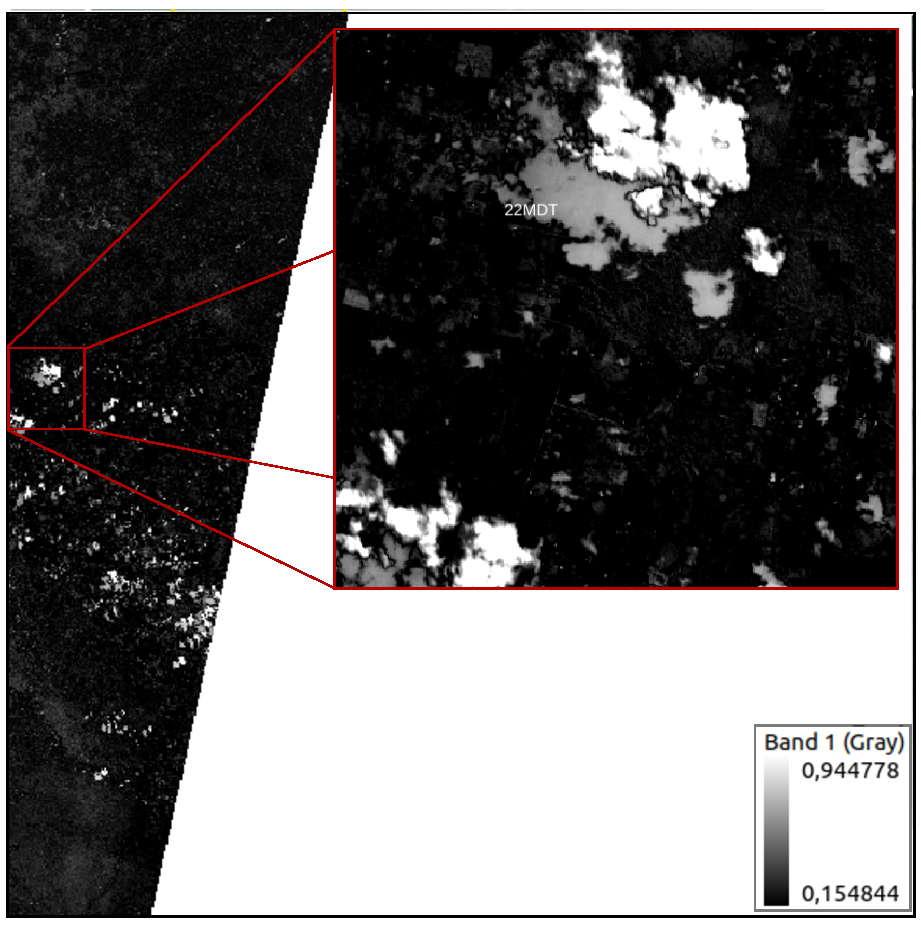
\includegraphics[width=2.5cm]{Figures/v3/20210513/222-error_map_with_zoom_roi.pdf}
% \end{tabular}
% \\
%    \centering
%     Binary masks
%     \begin{tabular}{ccc}
%     threshold = 0.3  & threshold =0.4 &  threshold = 0.5 \\
%     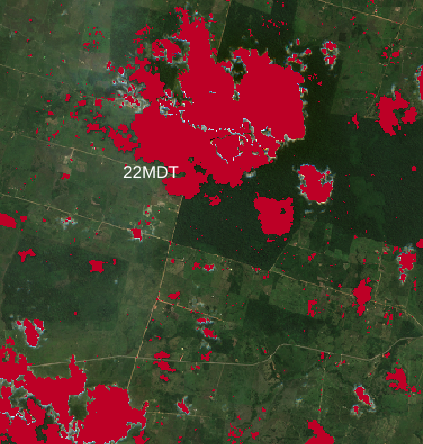
\includegraphics[width=3cm]{Figures/v3/20210513/binary_mask_umbral_03/zoom1.png}
%     &
%     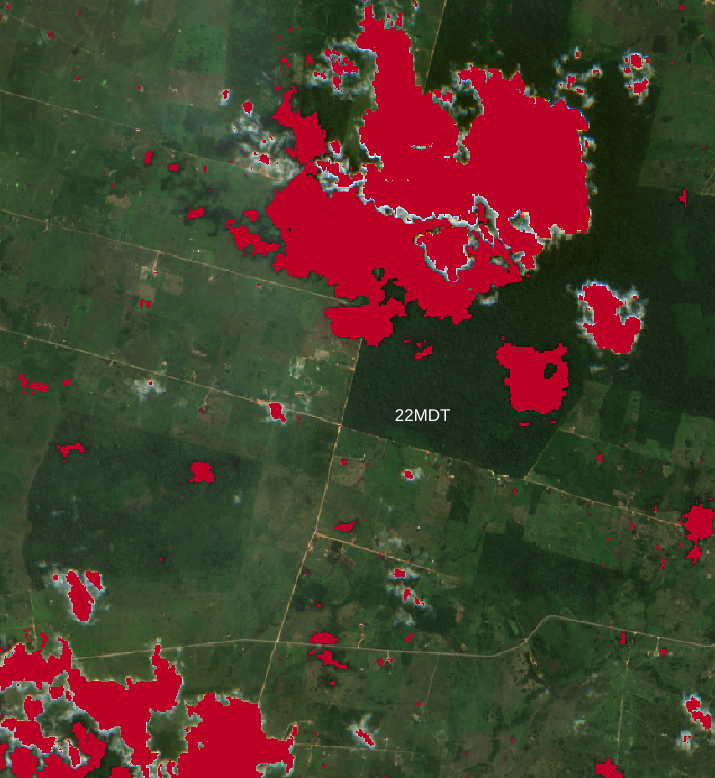
\includegraphics[width=2.9cm]{Figures/v3/20210513/binary_mask_umbral_04/zoom1.png}
%     &
%     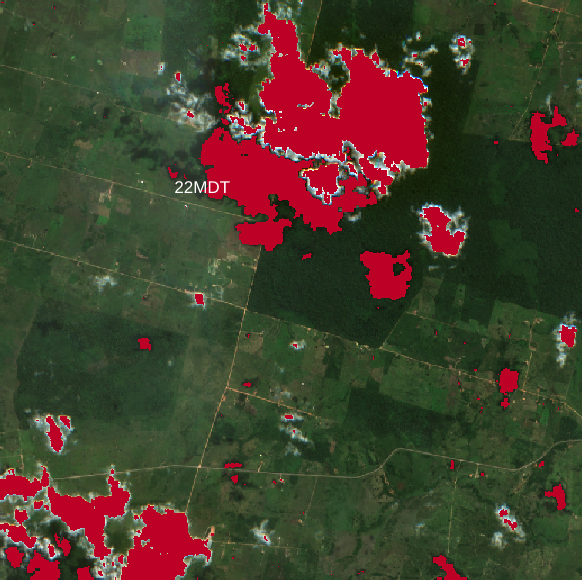
\includegraphics[width=3.2cm]{Figures/v3/20210513/binary_mask_umbral_05/33-binary_mask_zoom.png}
%     \end{tabular}
% \end{frame}

\begin{frame}{Date: 2021-05-13}
    \begin{tabular}{ccc}
        \multirow[c]{2}*[1cm]{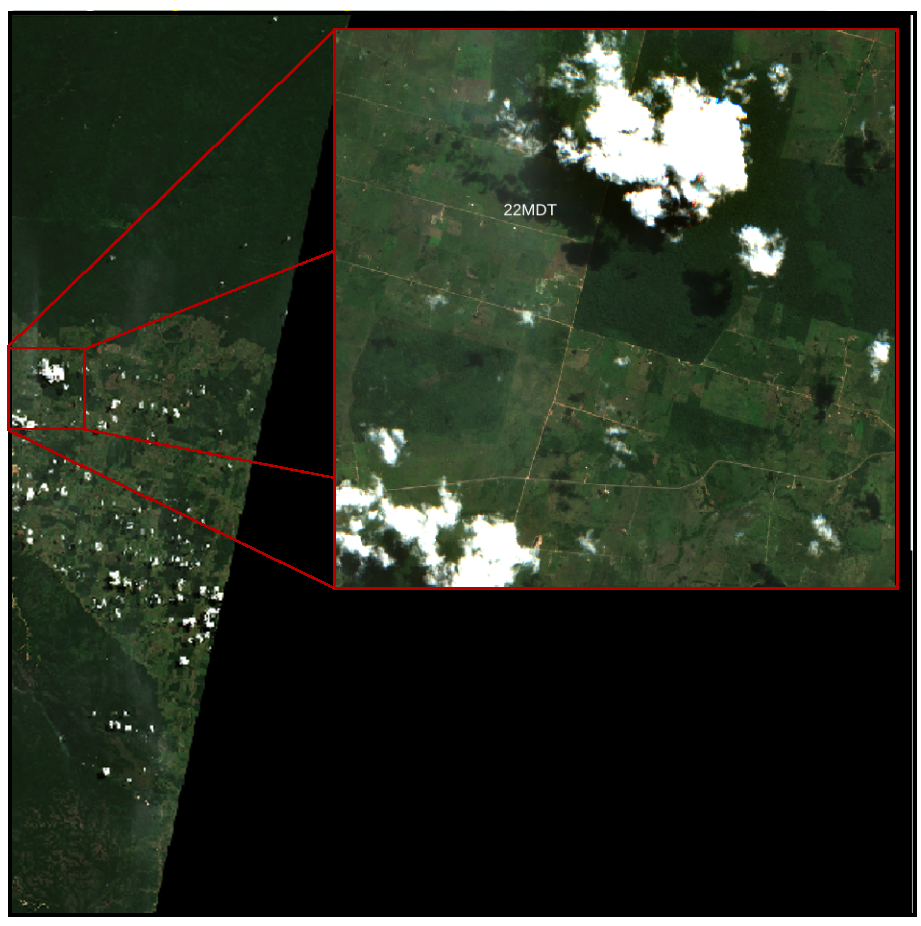
\includegraphics[width=.3\textwidth]{Figures/v3/20210513/111-TCI_with_zoom_roi.pdf}} & 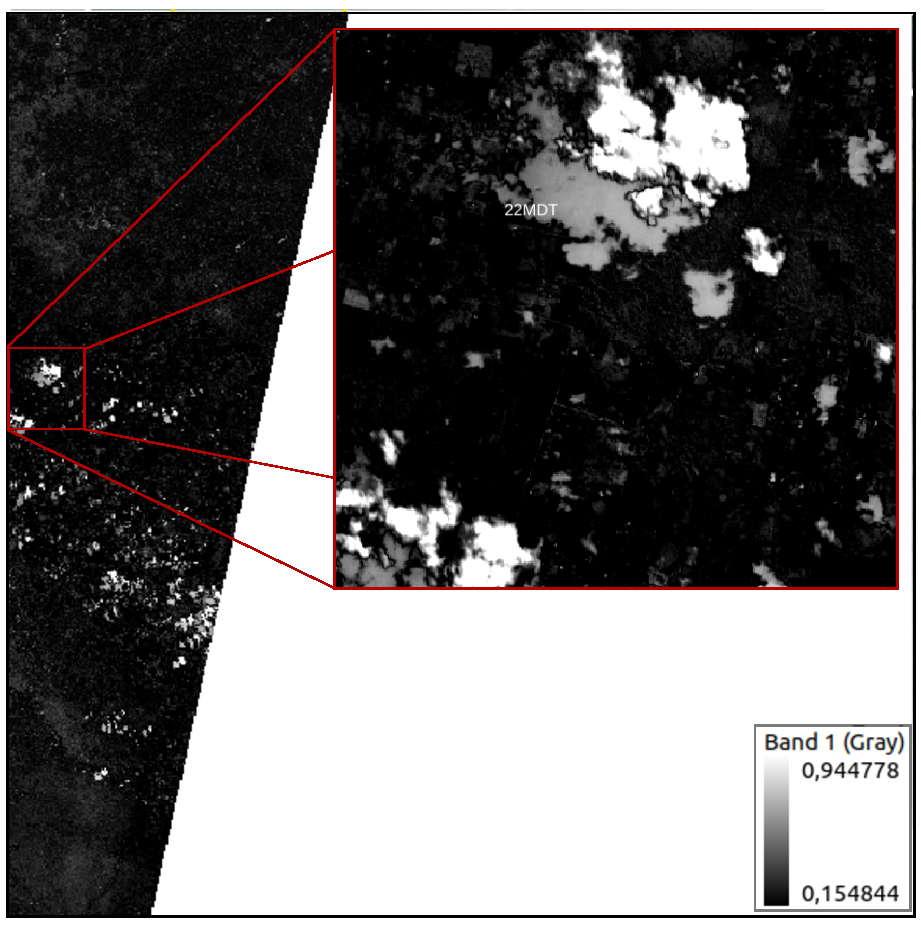
\includegraphics[width=3cm]{Figures/v3/20210513/222-error_map_with_zoom_roi.pdf} &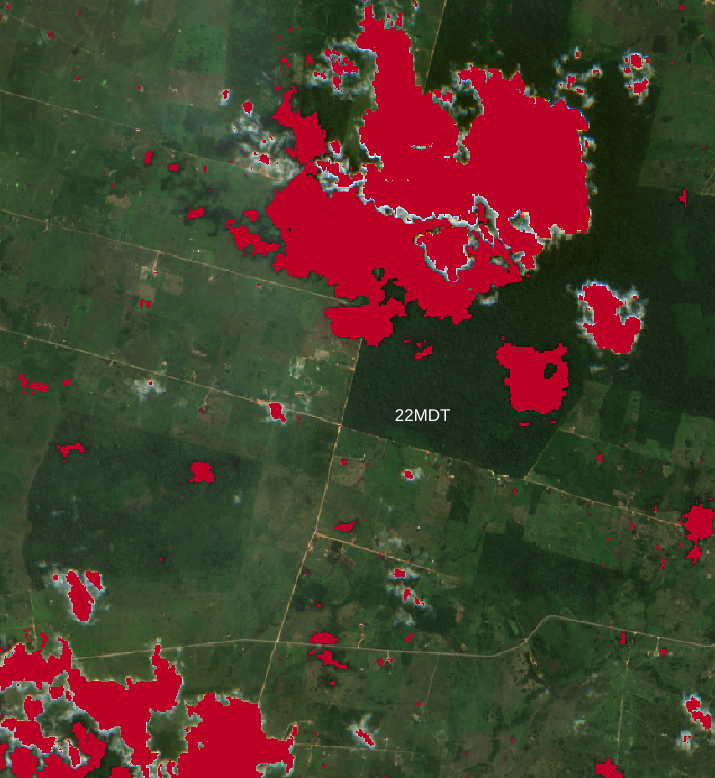
\includegraphics[width=2.7cm]{Figures/v3/20210513/binary_mask_umbral_04/zoom1.png}\\
        &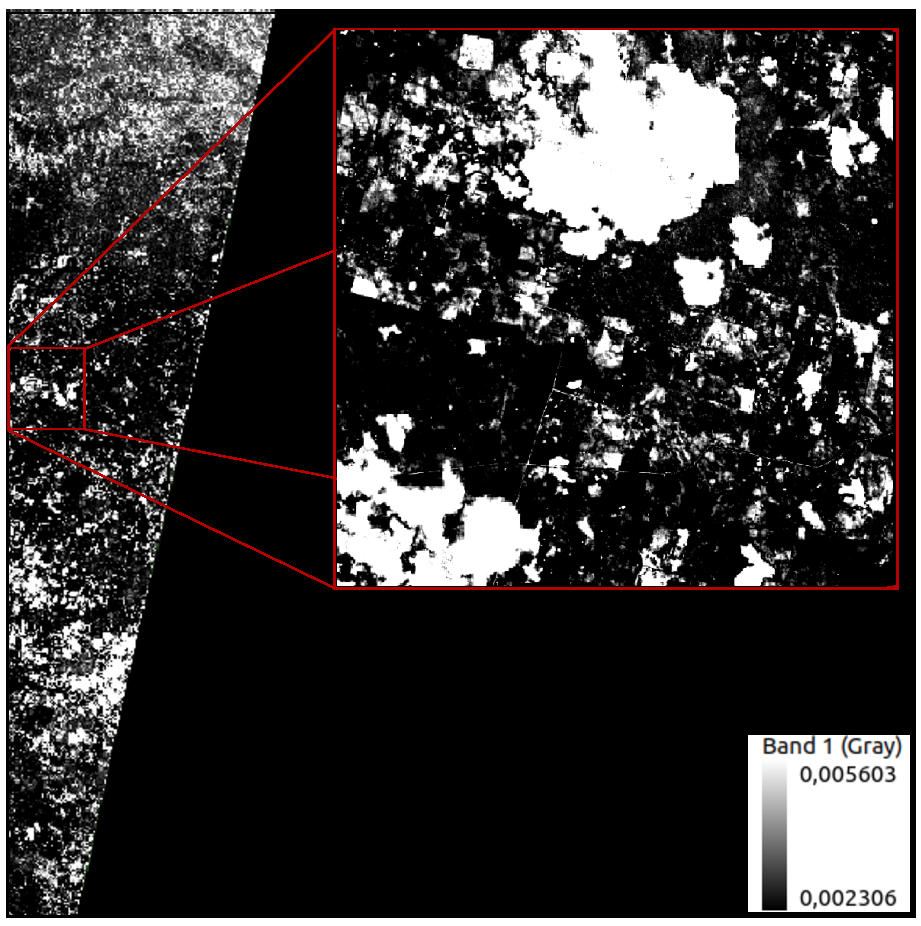
\includegraphics[width=3cm]{Figures/v4/20210513/error_map_BI_zoom1.pdf}&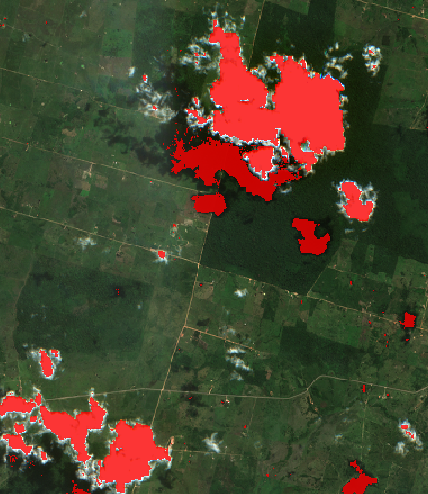
\includegraphics[width=2.7cm,height=3cm]{Figures/v4/20210513/zoom1_IB.png}
        \end{tabular}
\end{frame}

% \begin{frame}{Date: 2021-05-13}
%     \centering
%         \begin{tabular}{cc}
%         TCI & Error map\\
%         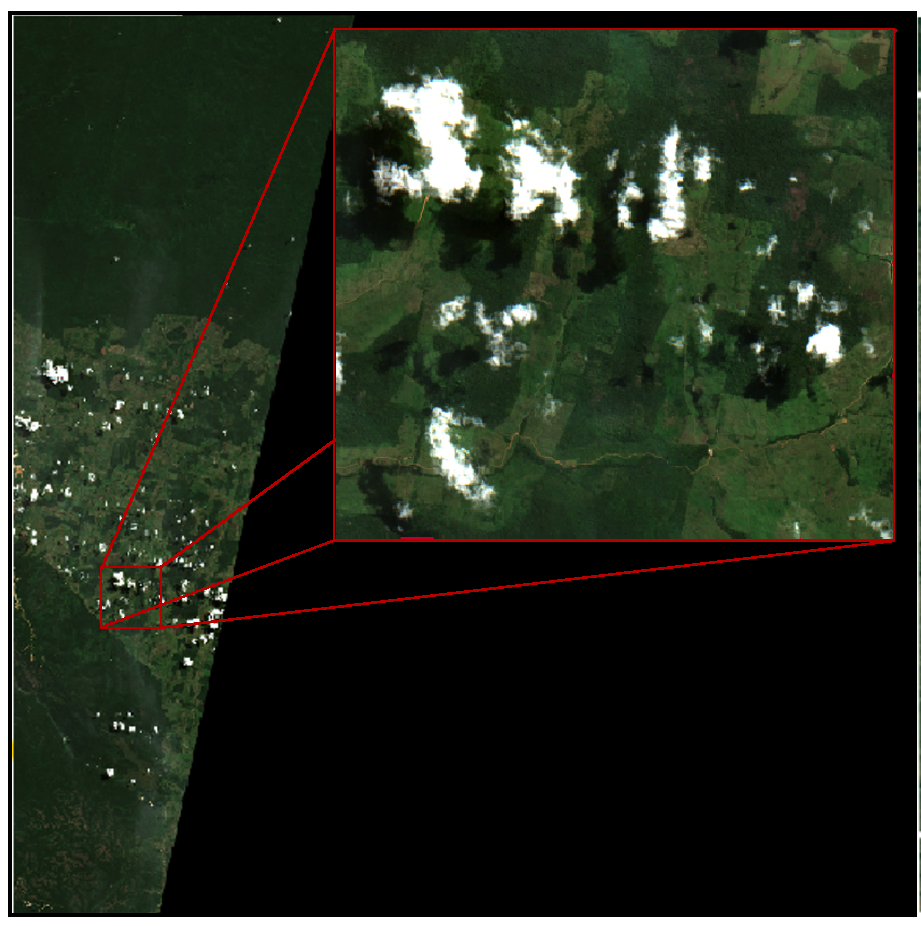
\includegraphics[width=3cm]{Figures/v3/20210513/111-TCI_with_zoom_roi2.pdf}
%         &
%         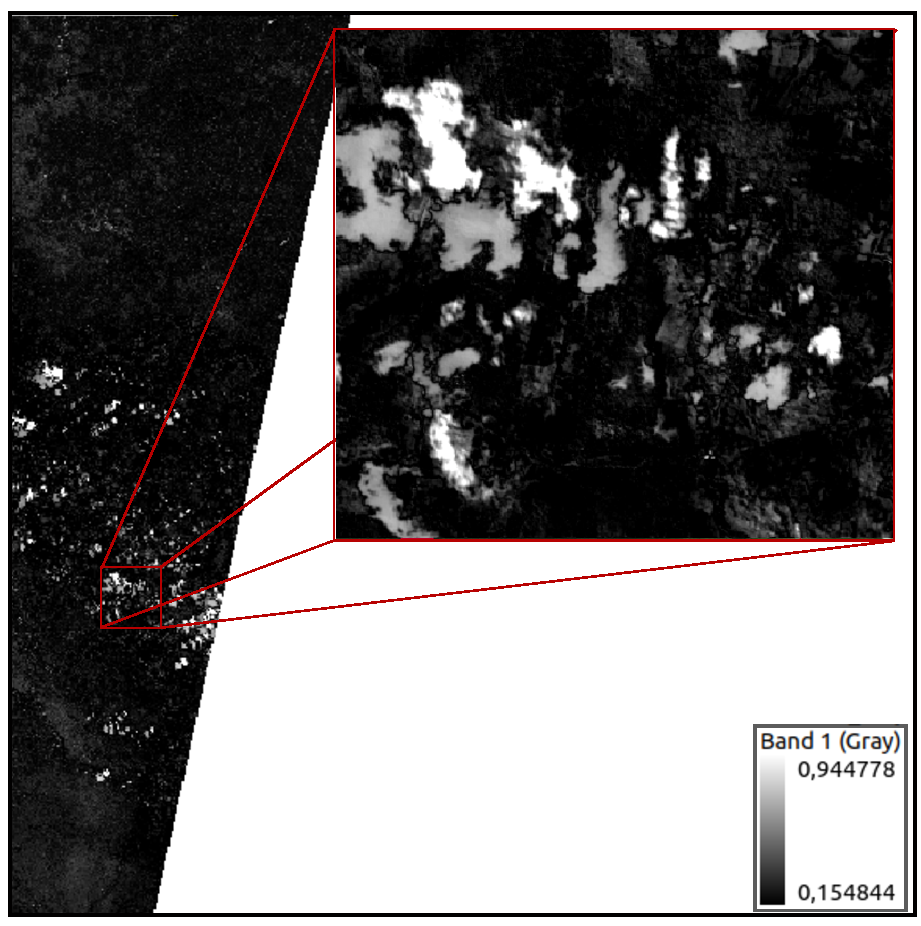
\includegraphics[width=3cm]{Figures/v3/20210513/222-error_map_with_zoom_roi2.pdf}
%     \end{tabular}
%     \\
%     \centering
%         Binary masks
%         \begin{tabular}{ccc}
%             threshold = 0.3  & threshold =0.4 &  threshold = 0.5 \\
%         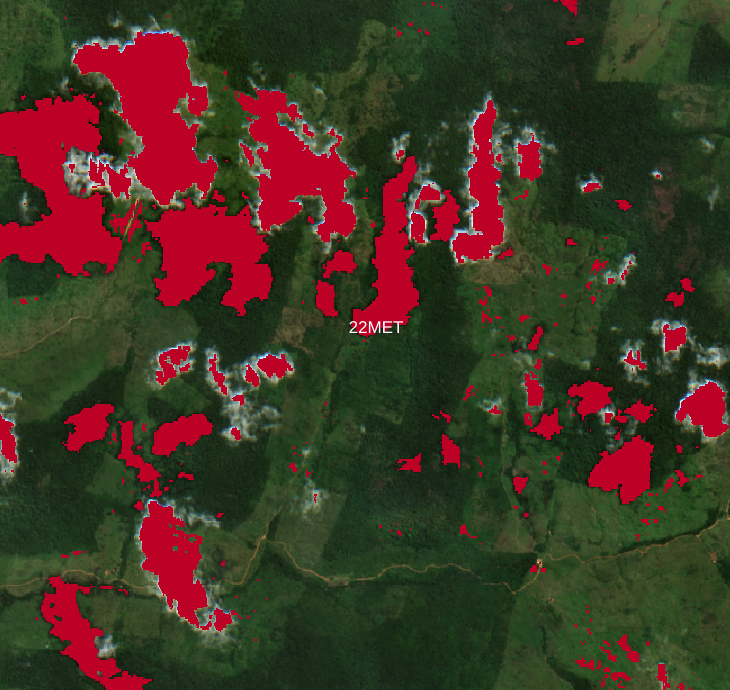
\includegraphics[width=2.8cm]{Figures/v3/20210513/binary_mask_umbral_03/zoom2.png}
%         &
%         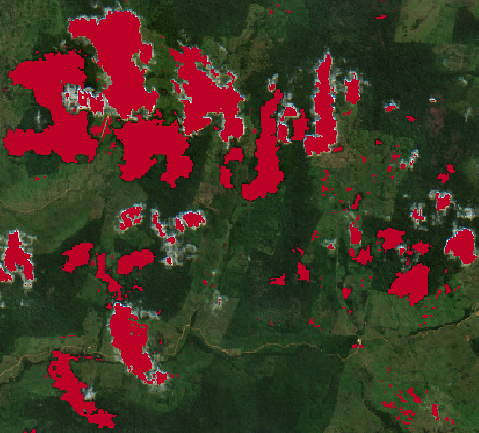
\includegraphics[width=2.9cm]{Figures/v3/20210513/binary_mask_umbral_04/zoom2.png}
%         &
%         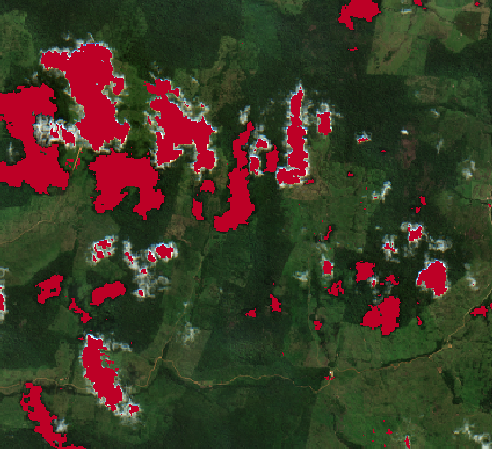
\includegraphics[width=2.9cm]{Figures/v3/20210513/binary_mask_umbral_05/33-binary_mask_zoom2.png}
%         \end{tabular}
%     \end{frame}

\begin{frame}{Date: 2021-05-13}
    \begin{tabular}{ccc}
        \multirow[c]{2}*[1cm]{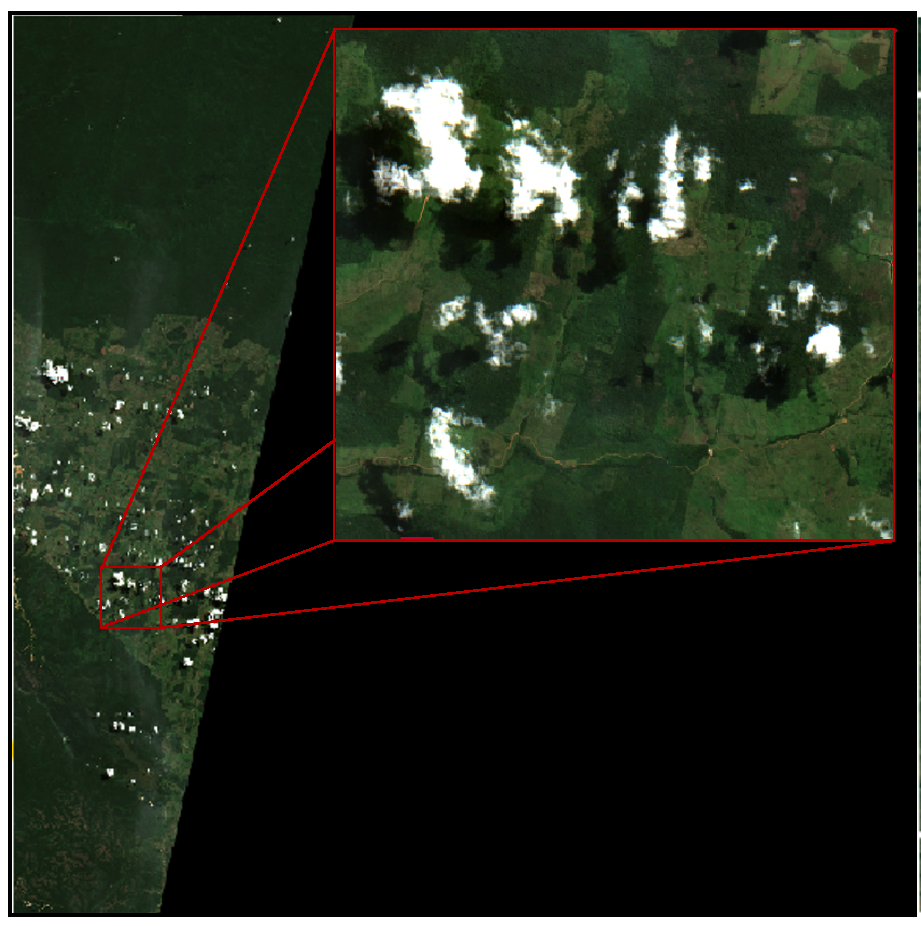
\includegraphics[width=.3\textwidth]{Figures/v3/20210513/111-TCI_with_zoom_roi2.pdf}} & 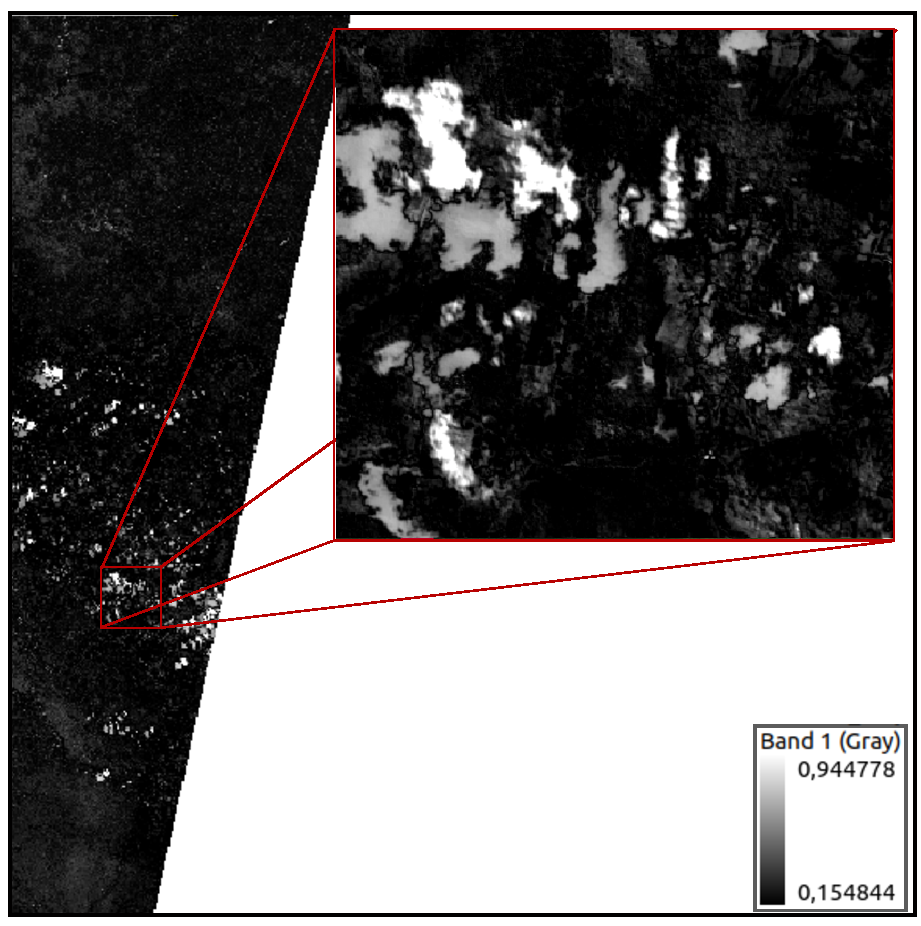
\includegraphics[width=3cm]{Figures/v3/20210513/222-error_map_with_zoom_roi2.pdf} &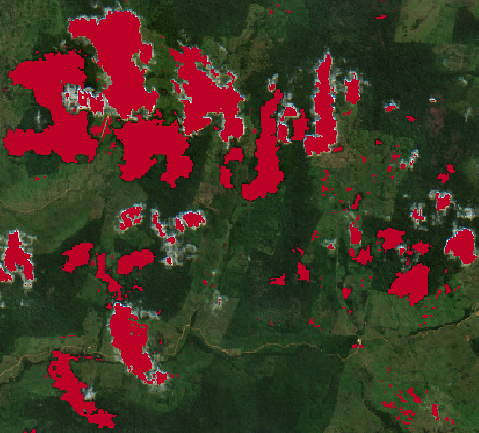
\includegraphics[width=2.7cm,height=3cm]{Figures/v3/20210513/binary_mask_umbral_04/zoom2.png}\\
        &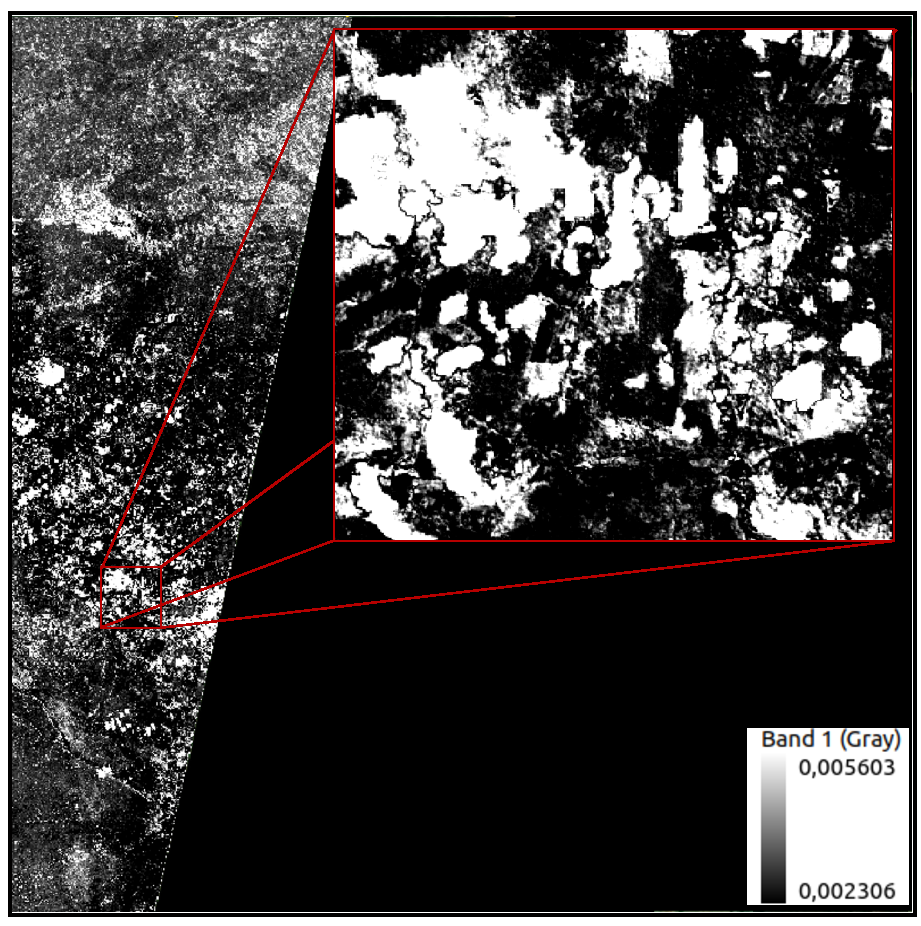
\includegraphics[width=3cm]{Figures/v4/20210513/error_map_BI_zoom2.pdf}&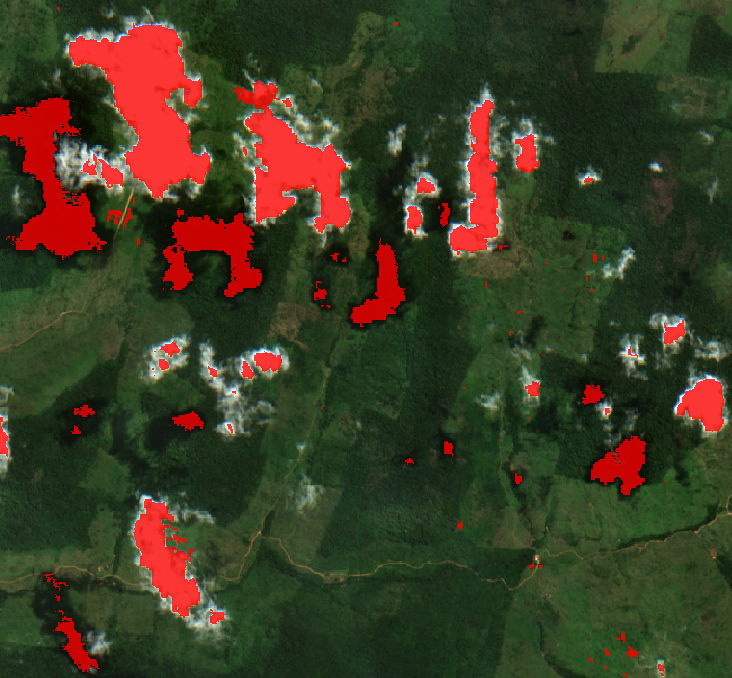
\includegraphics[width=2.7cm,height=3cm]{Figures/v4/20210513/zoom2_BI.png}
        \end{tabular}
\end{frame}

% \begin{frame}{Date: 2021-05-25}
% \centering
%     \begin{tabular}{cc}
%     TCI & Error map\\
%     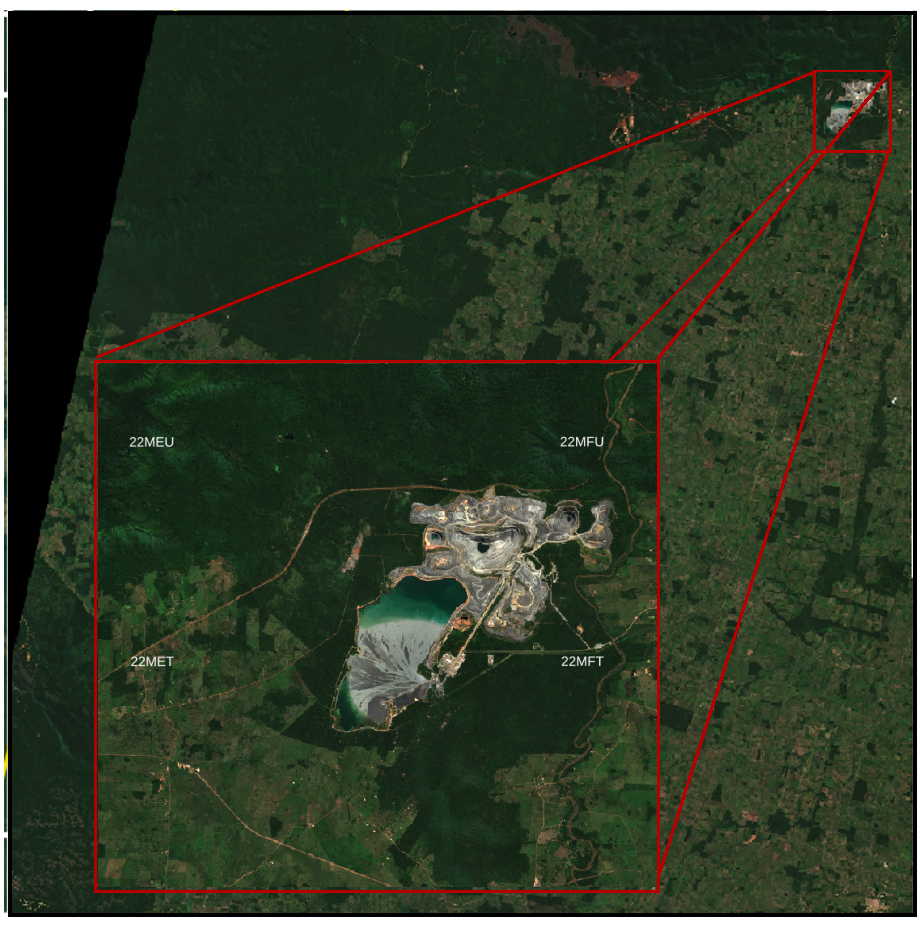
\includegraphics[width=3cm]{Figures/v3/20210525/TCI/TCI_zoom1.pdf}
%     &
%     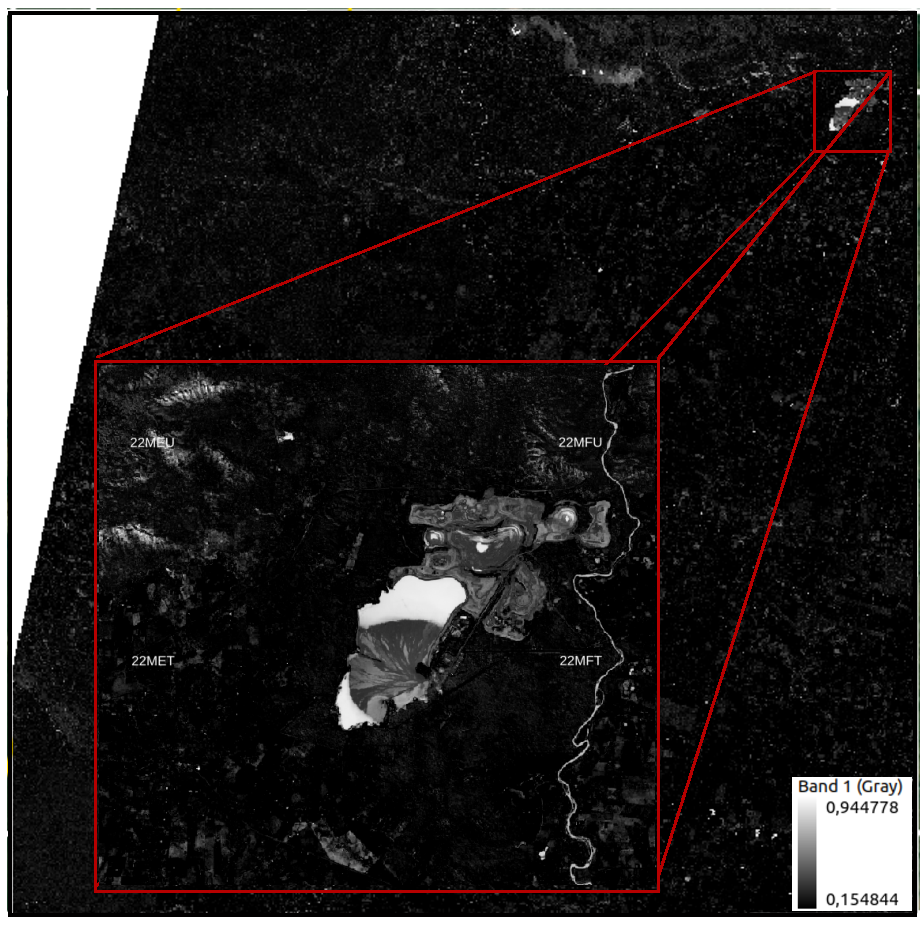
\includegraphics[width=3cm]{Figures/v3/20210525/error/error_zoom1.pdf}
% \end{tabular}
% \\
%    \centering
%     Binary masks
%     \begin{tabular}{ccc}
%         threshold = 0.3  & threshold =0.4 &  threshold = 0.5 \\
%     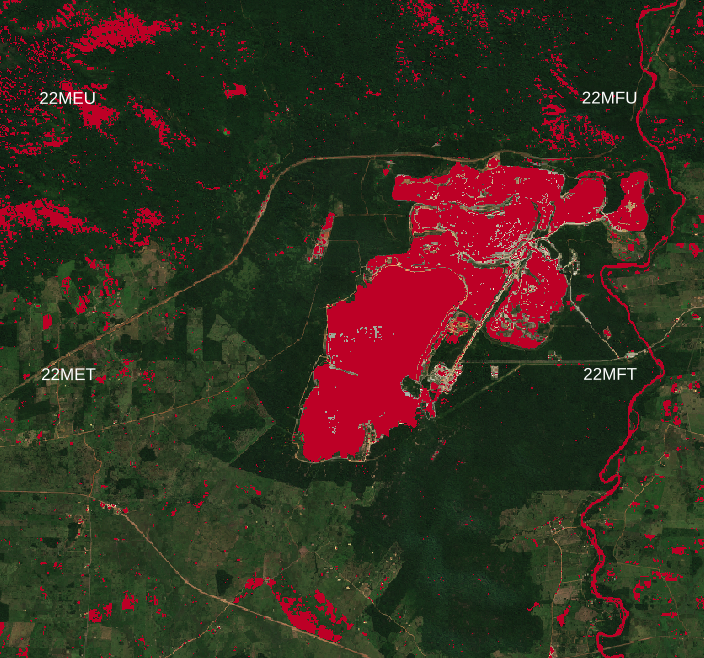
\includegraphics[width=3cm]{Figures/v3/20210525/umbral_03/zoom1.png}
%     &
%     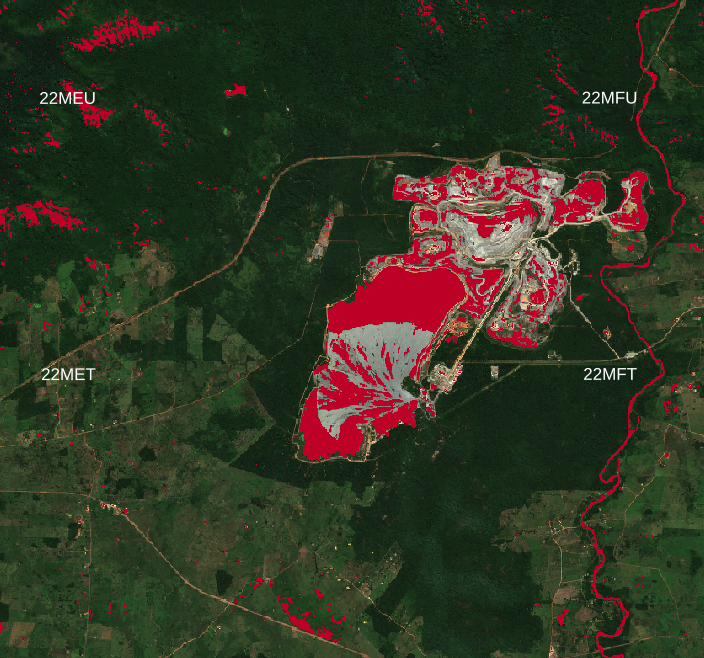
\includegraphics[width=3cm]{Figures/v3/20210525/umbral_04/zoom1.png}
%     &
%     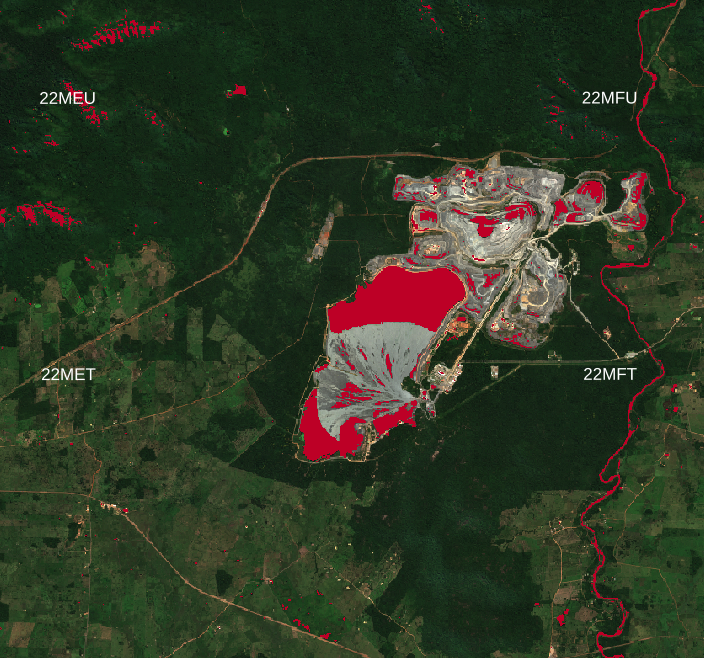
\includegraphics[width=3cm]{Figures/v3/20210525/umbral_05/zoom1.png}
%     \end{tabular}
% \end{frame}

\begin{frame}{Date: 2021-05-25}
    \begin{tabular}{ccc}
        \multirow[c]{2}*[1cm]{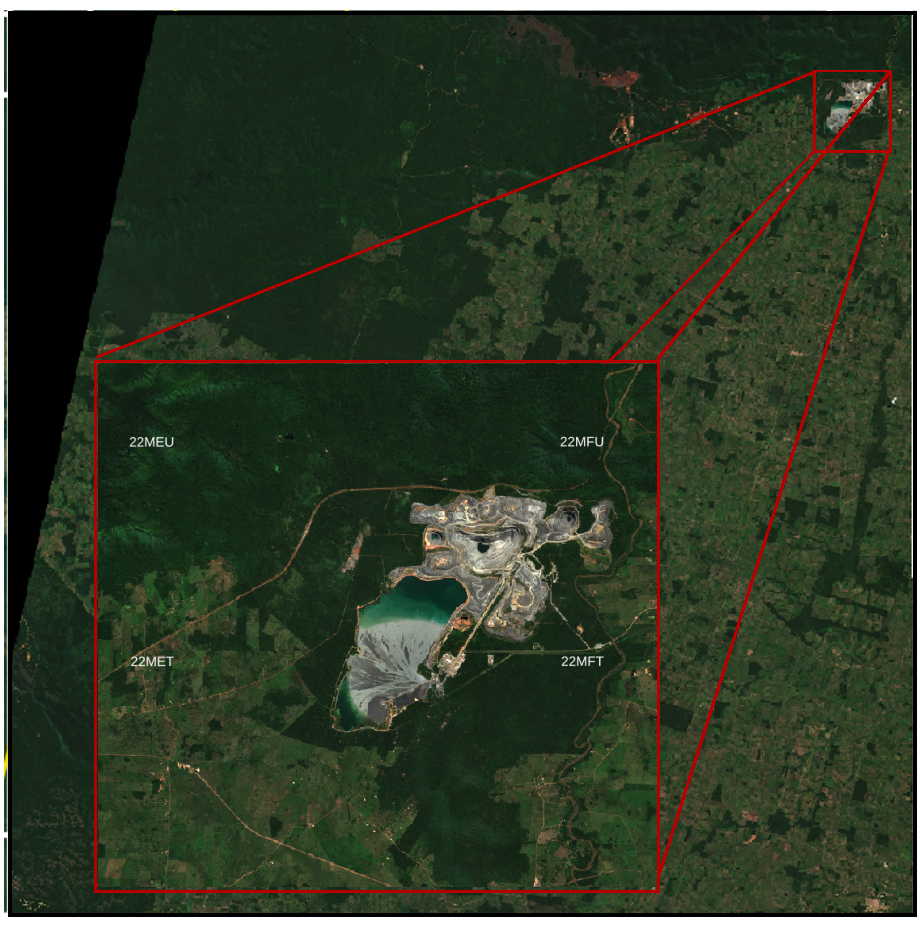
\includegraphics[width=.3\textwidth]{Figures/v3/20210525/TCI/TCI_zoom1.pdf}} & 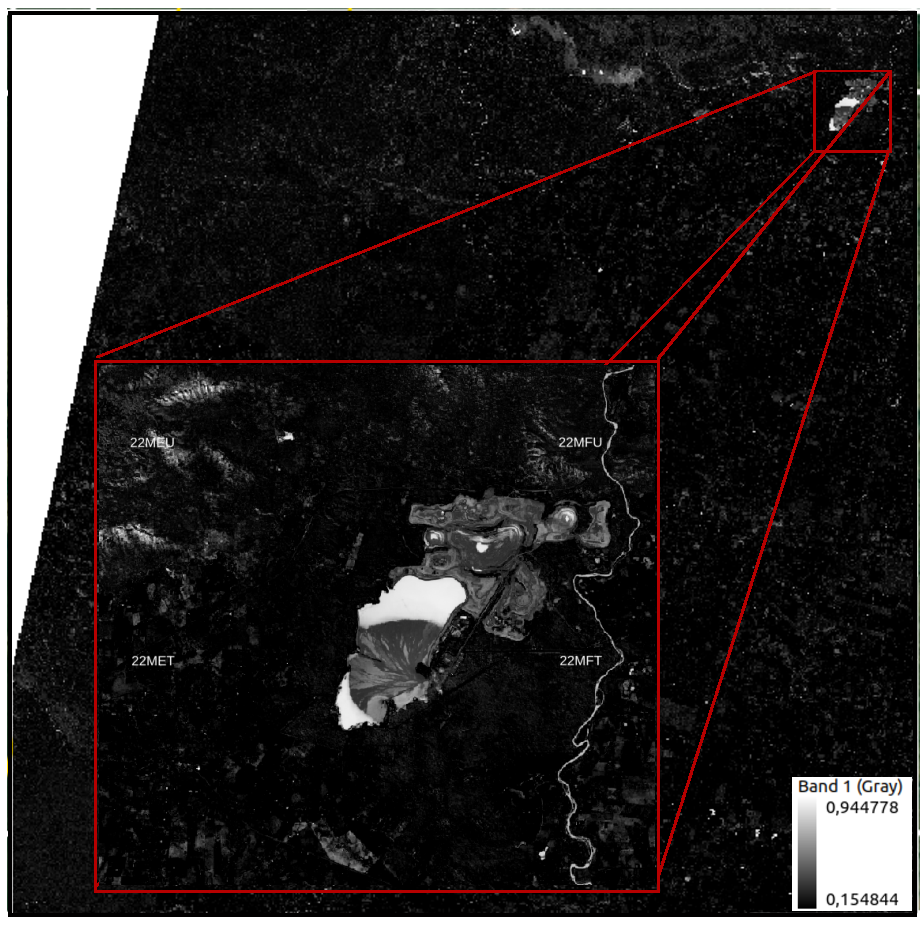
\includegraphics[width=3cm]{Figures/v3/20210525/error/error_zoom1.pdf} &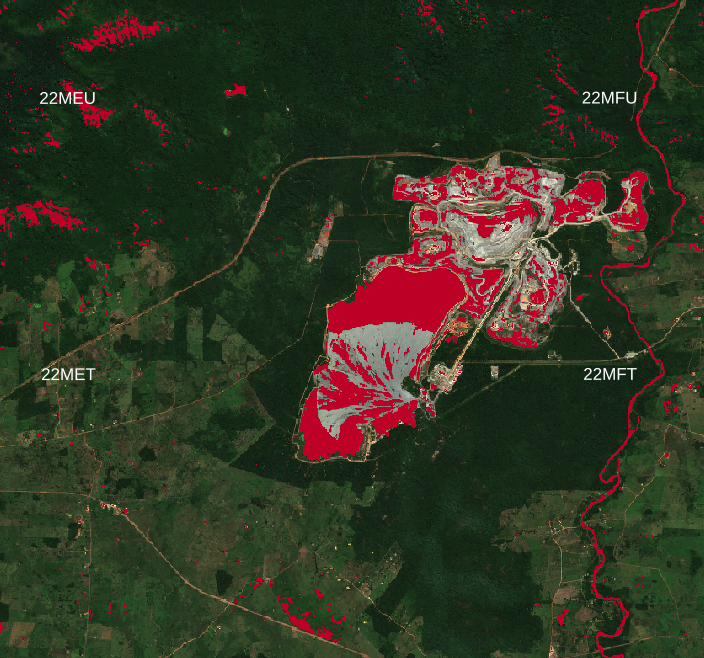
\includegraphics[width=2.7cm,height=3cm]{Figures/v3/20210525/umbral_04/zoom1.png}\\
        &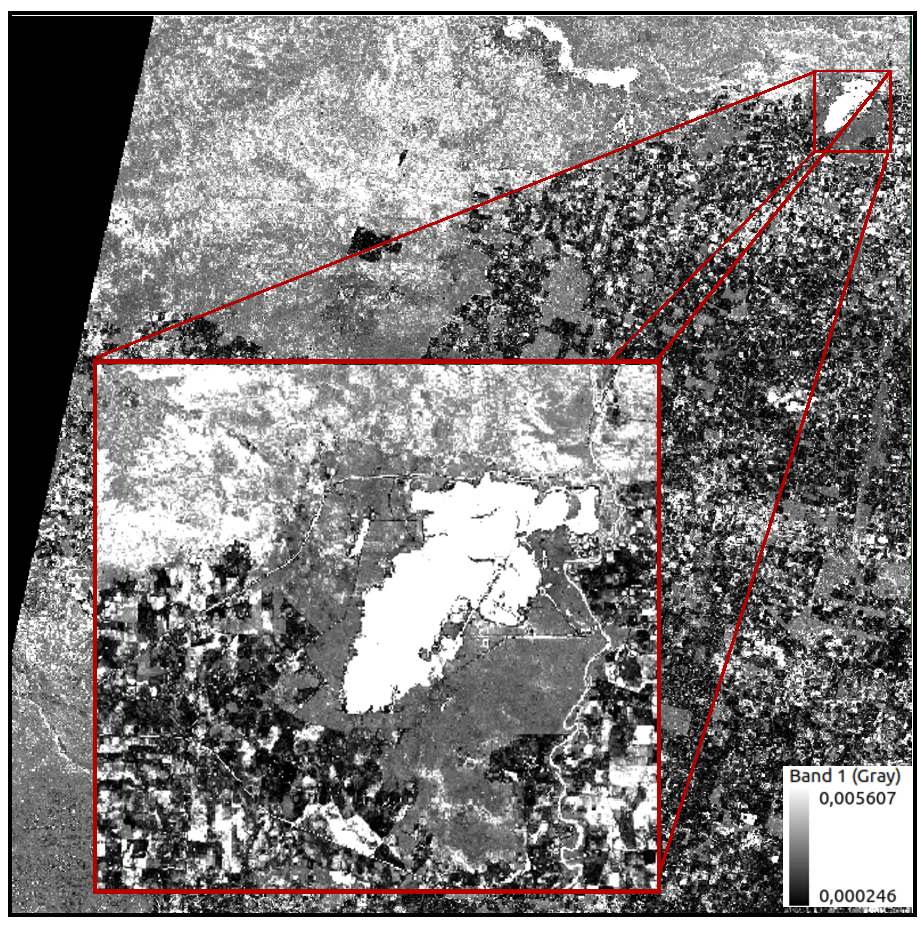
\includegraphics[width=3cm]{Figures/v4/20210525/error_zoom1.pdf}&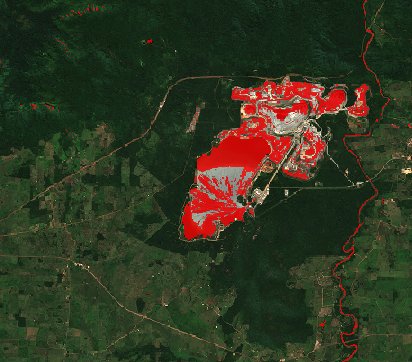
\includegraphics[width=2.7cm,height=3cm]{Figures/v4/20210525/zoom1_IB.png}
        \end{tabular}
\end{frame}


% \begin{frame}{Date: 2021-05-25}
%     \centering
%         \begin{tabular}{cc}
%         TCI & Error map\\
%         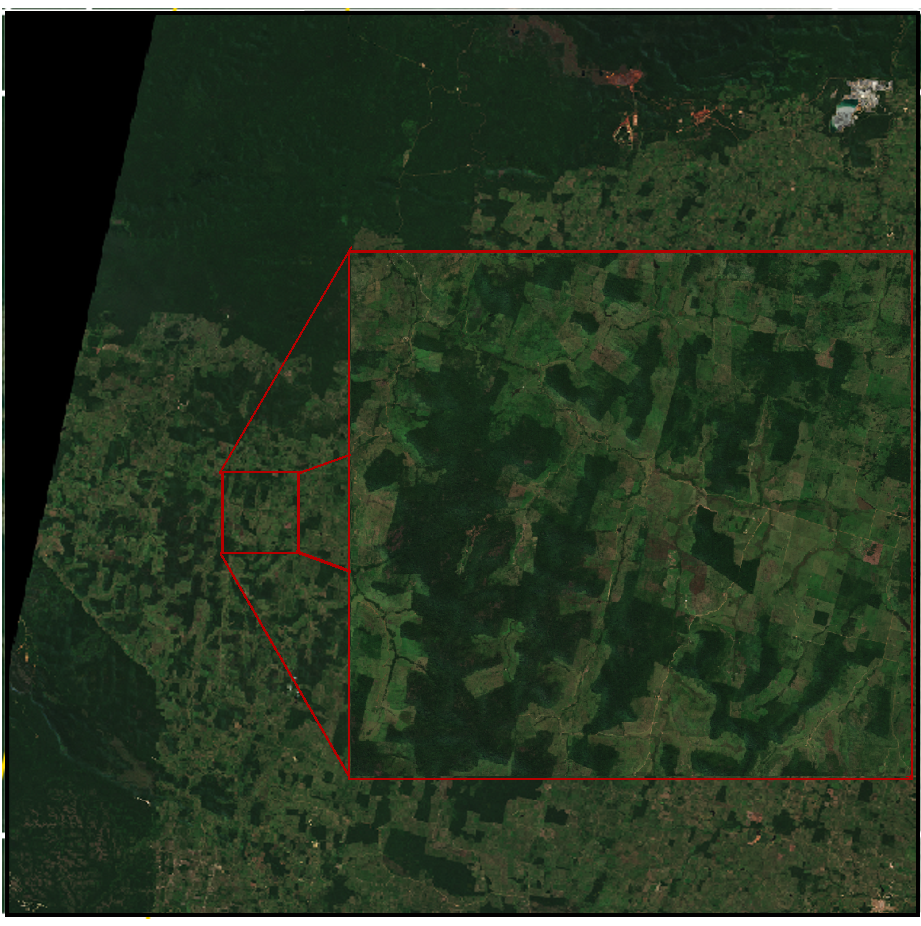
\includegraphics[width=3cm]{Figures/v3/20210525/TCI/TCI_zoom2.pdf}
%         &
%         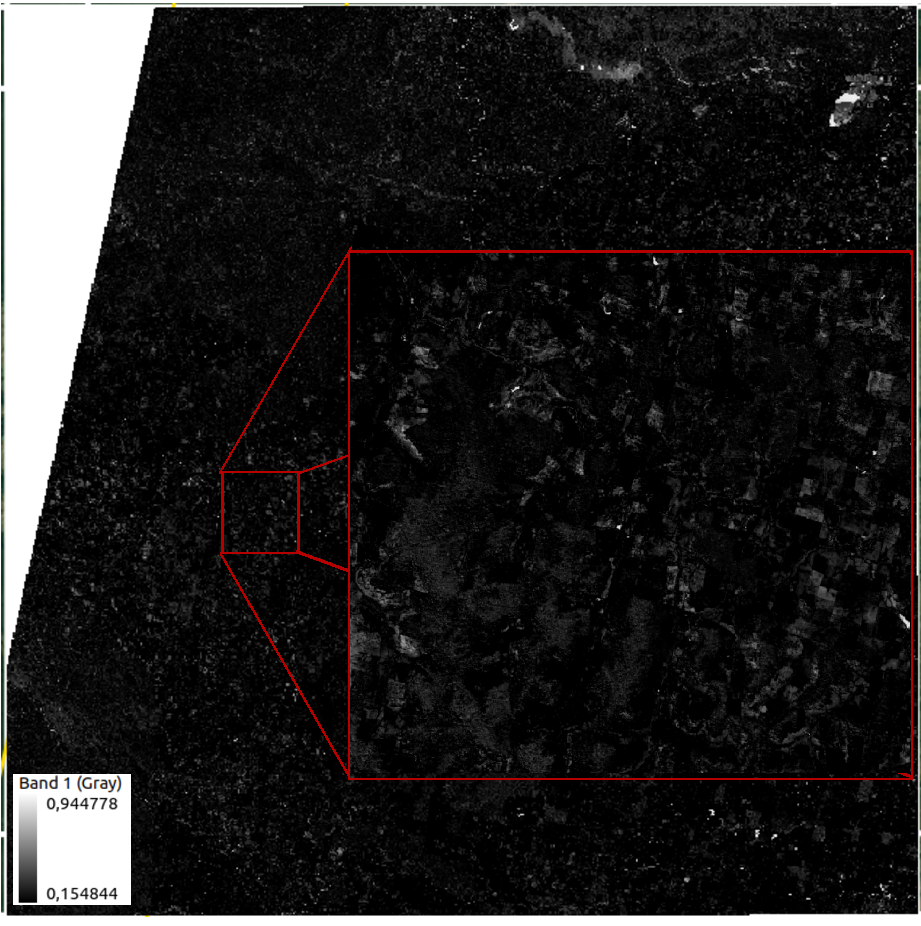
\includegraphics[width=3cm]{Figures/v3/20210525/error/error_zoom2.pdf}
%     \end{tabular}
%     \\
%     \centering
%      Binary masks
%         \begin{tabular}{ccc}
%             threshold = 0.3  & threshold =0.4 &  threshold = 0.5 \\
%         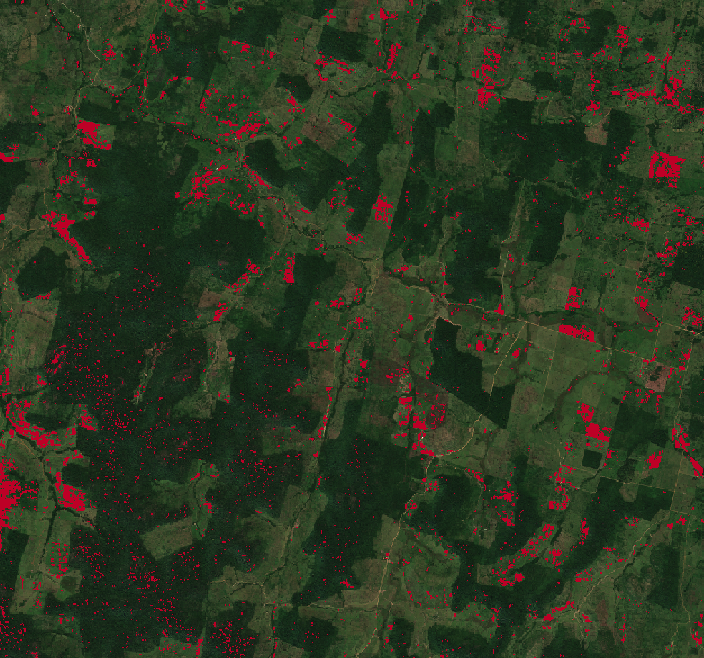
\includegraphics[width=3cm]{Figures/v3/20210525/umbral_03/zoom2.png}
%         &
%         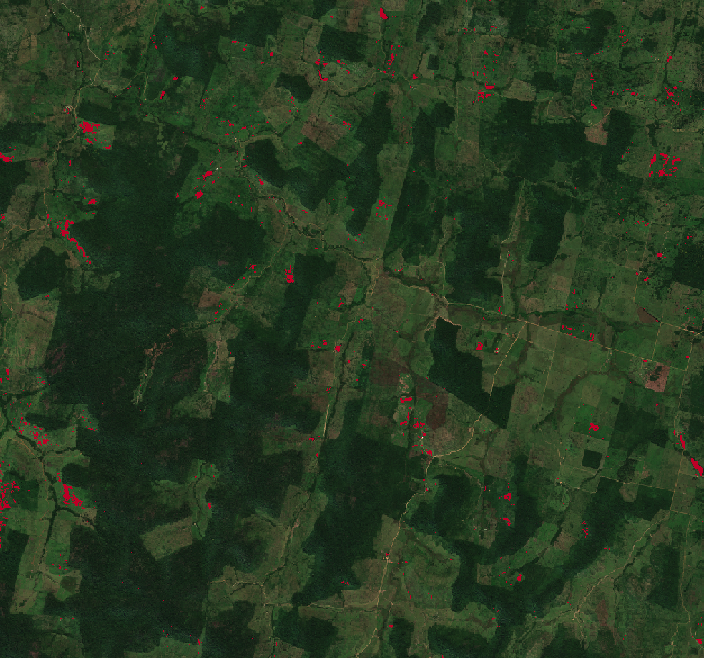
\includegraphics[width=3cm]{Figures/v3/20210525/umbral_04/zoom2.png}
%         &
%         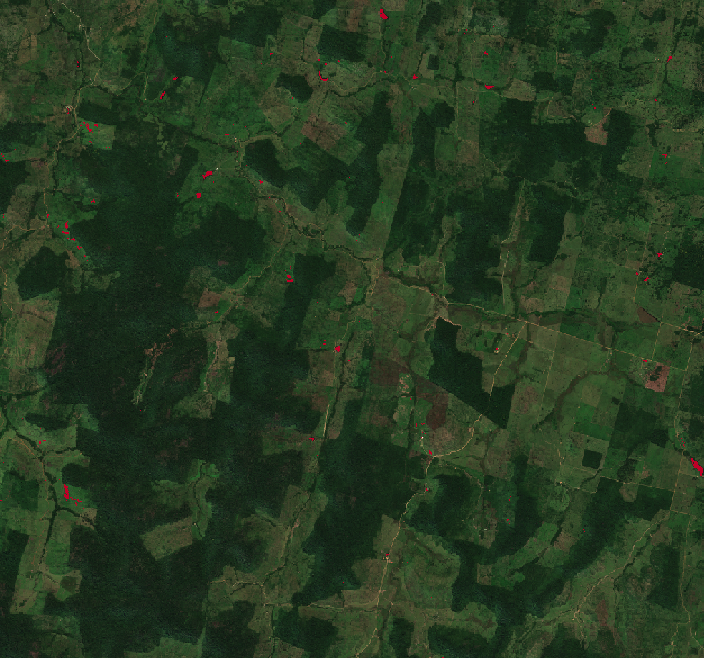
\includegraphics[width=3cm]{Figures/v3/20210525/umbral_05/zoom2.png}
%         \end{tabular}
%     \end{frame}

\begin{frame}{Date: 2021-05-25}
    \begin{tabular}{ccc}
        \multirow[c]{2}*[1cm]{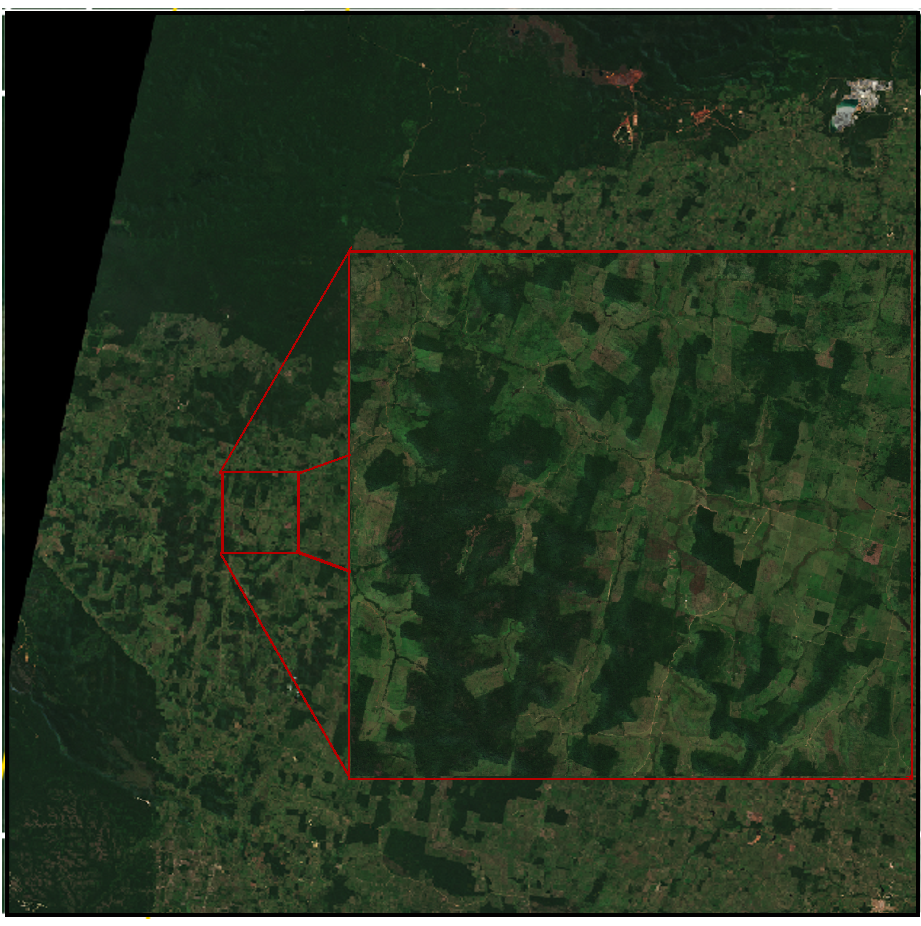
\includegraphics[width=.3\textwidth]{Figures/v3/20210525/TCI/TCI_zoom2.pdf}} & 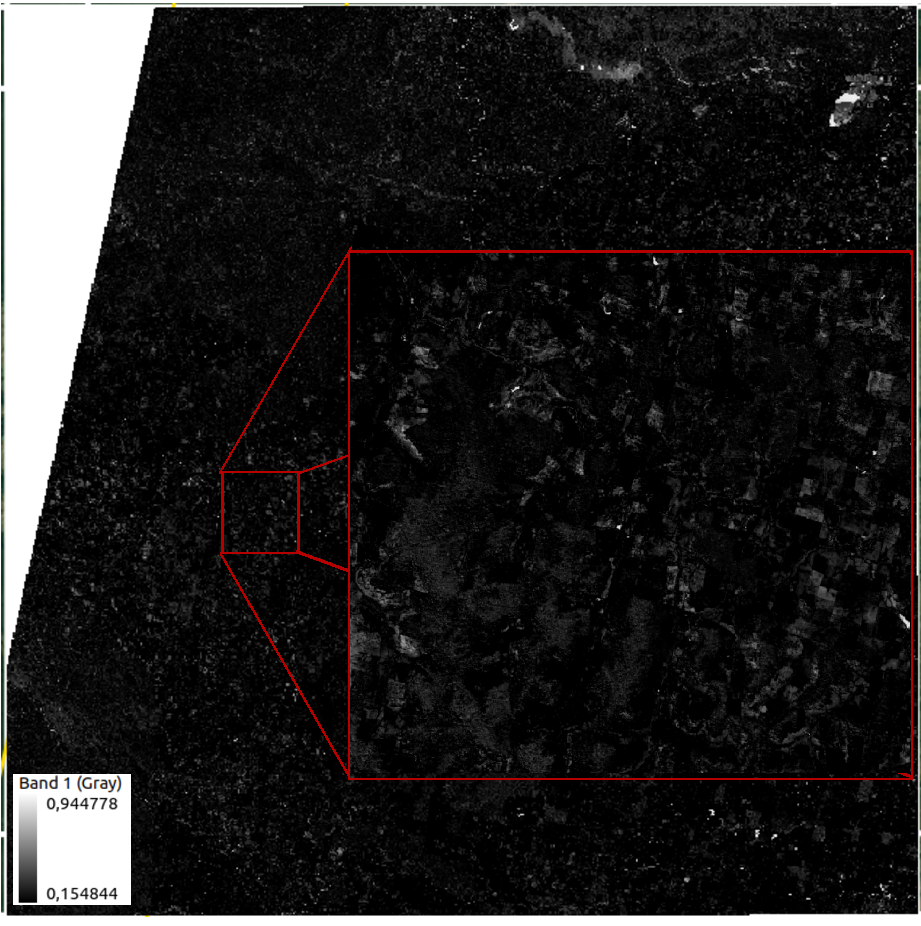
\includegraphics[width=3cm]{Figures/v3/20210525/error/error_zoom2.pdf} &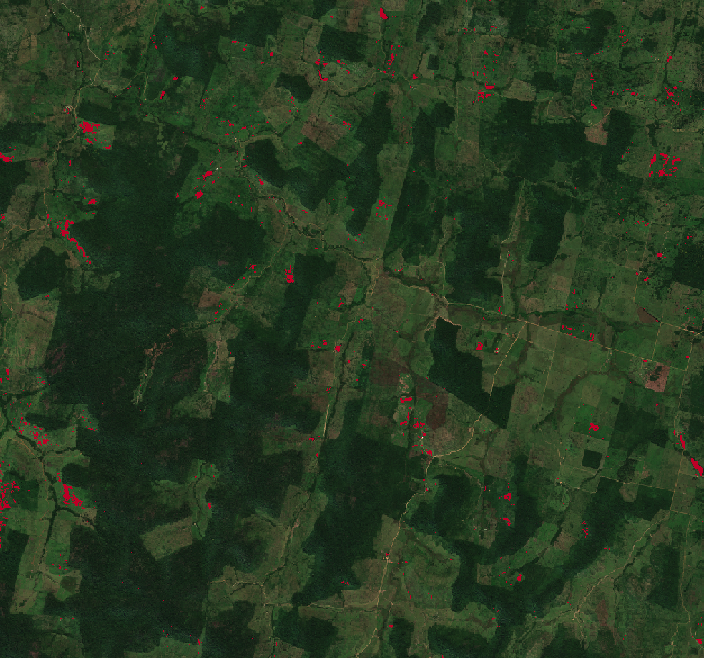
\includegraphics[width=2.7cm,height=3cm]{Figures/v3/20210525/umbral_04/zoom2.png}\\
        &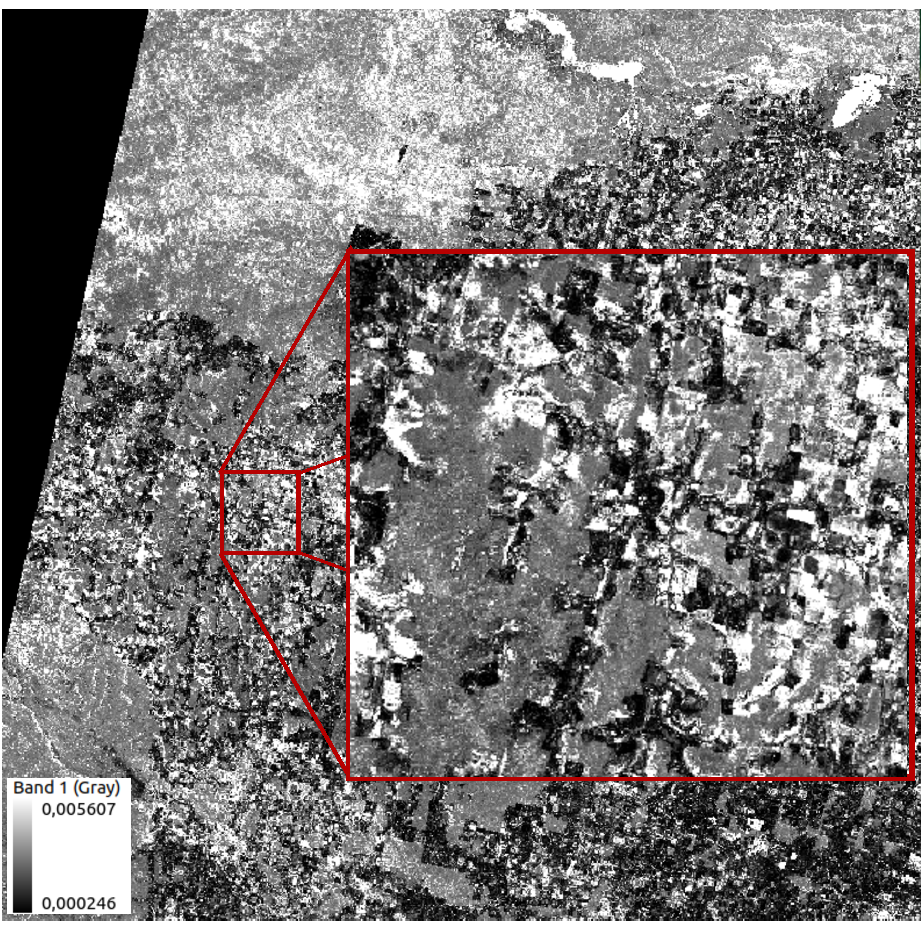
\includegraphics[width=3cm]{Figures/v4/20210525/error_zoom2.pdf}&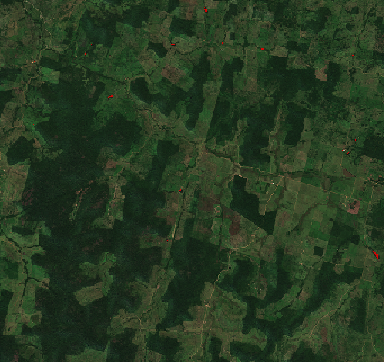
\includegraphics[width=2.7cm,height=3cm]{Figures/v4/20210525/zoom2_BI.png}
        \end{tabular}
\end{frame}

% \begin{frame}{Date: 2021-05-28}
%     \centering
%         \begin{tabular}{cc}
%         TCI & Error map\\
%         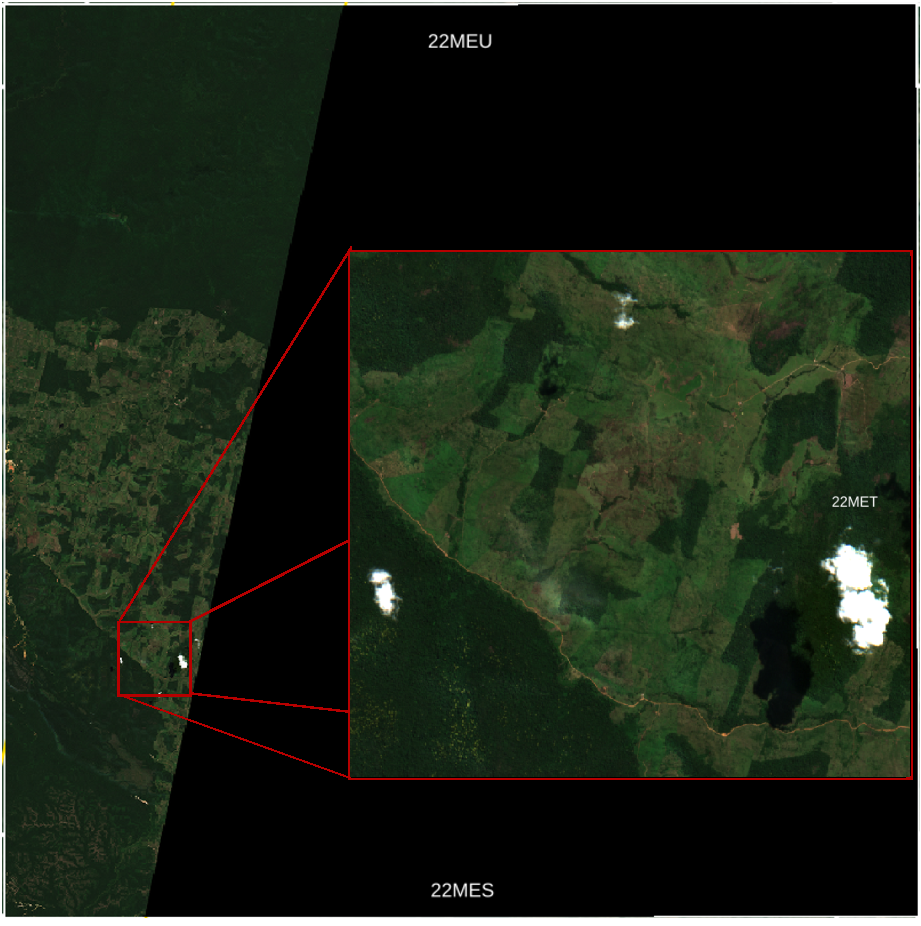
\includegraphics[width=3cm]{Figures/v3/20210528/TCI/TCI_zoom1.pdf}
%         &
%         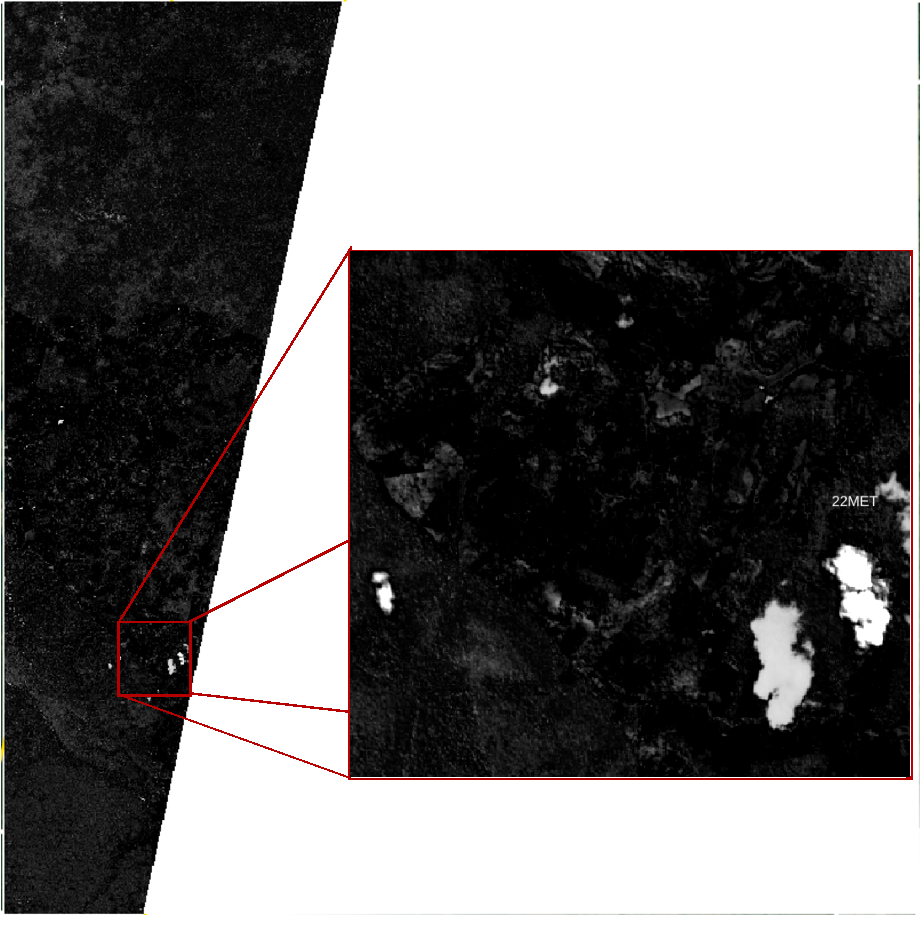
\includegraphics[width=3cm]{Figures/v3/20210528/error_map/error_zoom1.pdf}
%     \end{tabular}
%     \\
%    \centering
%     Binary masks
%         \begin{tabular}{ccc}
%             threshold = 0.3  & threshold =0.4 &  threshold = 0.5 \\
%         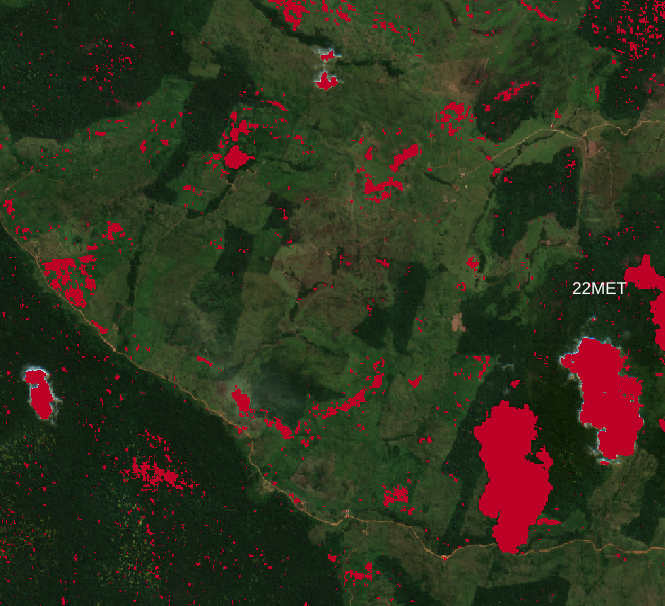
\includegraphics[width=3cm]{Figures/v3/20210528/umbral_03/zoom1.png}
%         &
%         \includegraphics[width=3cm]{Figures/v3/20210528/umbral_04/zoom1.png}
%         &
%         \includegraphics[width=3cm]{Figures/v3/20210528/umbral_05/zoom1.png}
%         \end{tabular}
% \end{frame}

\begin{frame}{Date: 2021-05-28}
    \begin{tabular}{ccc}
        \multirow[c]{2}*[1cm]{\includegraphics[width=.3\textwidth]{Figures/v3/20210528/TCI/TCI_zoom1.pdf}} & \includegraphics[width=3cm]{Figures/v3/20210528/error_map/error_zoom1.pdf} &\includegraphics[width=2.7cm,height=3cm]{Figures/v3/20210528/umbral_04/zoom1.png}\\
        &\includegraphics[width=3cm]{Figures/v4/20210528/error_zoom1.pdf}&\includegraphics[width=2.7cm,height=3cm]{Figures/v4/20210528/zoom1_IB.png}
        \end{tabular}
\end{frame}

% \begin{frame}{Date: 2021-05-28}
%     \centering
%         \begin{tabular}{cc}
%         TCI & Error map\\
%         \includegraphics[width=3cm]{Figures/v3/20210528/TCI/TCI_zoom2.pdf}
%         &
%         \includegraphics[width=3cm]{Figures/v3/20210528/error_map/error_zoom2.pdf}
%     \end{tabular}
%     \\
%     \centering
%      Binary masks
%         \begin{tabular}{ccc}
%             threshold = 0.3  & threshold =0.4 &  threshold = 0.5 \\
%         \includegraphics[width=3cm]{Figures/v3/20210528/umbral_03/zoom2.png}
%         &
%         \includegraphics[width=3cm]{Figures/v3/20210528/umbral_04/zoom2.png}
%         &
%         \includegraphics[width=3cm]{Figures/v3/20210528/umbral_05/zoom2.png}
%         \end{tabular}
% \end{frame}

\begin{frame}{Date: 2021-05-28}
    \begin{tabular}{ccc}
        \multirow[c]{2}*[1cm]{\includegraphics[width=.3\textwidth]{Figures/v3/20210528/TCI/TCI_zoom2.pdf}} & \includegraphics[width=3cm]{Figures/v3/20210528/error_map/error_zoom2.pdf} &\includegraphics[width=2.7cm,height=3cm]{Figures/v3/20210528/umbral_04/zoom2.png}\\
        &\includegraphics[width=3cm]{Figures/v4/20210528/error_zoom2.pdf}&\includegraphics[width=2.7cm,height=3cm]{Figures/v4/20210528/zoom2_BI.png}
        \end{tabular}
\end{frame}

% \begin{frame}{Date: 2021-05-30}
%     \centering
%         \begin{tabular}{cc}
%         TCI & Error map\\
%         \includegraphics[width=2.8cm]{Figures/v3/20210530/TCI/tci_zoom1.pdf}
%         &
%         \includegraphics[width=2.8cm]{Figures/v3/20210530/error_map/error_zoom1.pdf}
%     \end{tabular}
%     \\
%    \centering
%     Binary masks
%         \begin{tabular}{ccc}
%             threshold = 0.3  & threshold =0.4 &  threshold = 0.5 \\
%         \includegraphics[width=3cm]{Figures/v3/20210530/umbral_03/zoom1.png}
%         &
%         \includegraphics[width=3cm]{Figures/v3/20210530/umbral_04/zoom1.png}
%         &
%         \includegraphics[width=3cm]{Figures/v3/20210530/umbral_05/zoom1.png}
%         \end{tabular}
% \end{frame}

\begin{frame}{Date: 2021-05-30}
    \begin{tabular}{ccc}
        \multirow[c]{2}*[1cm]{\includegraphics[width=.3\textwidth]{Figures/v3/20210530/TCI/tci_zoom1.pdf}} & \includegraphics[width=3cm]{Figures/v3/20210530/error_map/error_zoom1.pdf} &\includegraphics[width=2.7cm,height=3cm]{Figures/v3/20210530/umbral_04/zoom1.png}\\
        &\includegraphics[width=3cm]{Figures/v4/20210530/error_zoom1.pdf}&\includegraphics[width=2.7cm,height=3cm]{Figures/v4/20210530/zoom1_BI.png}
        \end{tabular}
\end{frame}

% \begin{frame}{Date: 2021-05-30}
%     \centering
%         \begin{tabular}{cc}
%         TCI & Error map\\
%         \includegraphics[width=2.8cm]{Figures/v3/20210530/TCI/tci_zoom2.pdf}
%         &
%         \includegraphics[width=2.8cm]{Figures/v3/20210530/error_map/error_zoom2.pdf}
%     \end{tabular}
%     \\
%    \centering
%     Binary masks
%         \begin{tabular}{ccc}
%             threshold = 0.3  & threshold =0.4 &  threshold = 0.5 \\
%         \includegraphics[width=3cm]{Figures/v3/20210530/umbral_03/zoom2.png}
%         &
%         \includegraphics[width=3cm]{Figures/v3/20210530/umbral_04/zoom2.png}
%         &
%         \includegraphics[width=3cm]{Figures/v3/20210530/umbral_05/zoom2.png}
%         \end{tabular}
% \end{frame}

\begin{frame}{Date: 2021-05-30}
    \begin{tabular}{ccc}
        \multirow[c]{2}*[1cm]{\includegraphics[width=.3\textwidth]{Figures/v3/20210530/TCI/tci_zoom2.pdf}} & \includegraphics[width=3cm]{Figures/v3/20210530/error_map/error_zoom2.pdf} &\includegraphics[width=2.7cm,height=3cm]{Figures/v3/20210530/umbral_04/zoom2.png}\\
        &\includegraphics[width=3cm]{Figures/v4/20210530/error_zoom2.pdf}&\includegraphics[width=2.7cm,height=3cm]{Figures/v4/20210530/zoom2_BI.png}
        \end{tabular}
\end{frame}

% \begin{frame}{Date: 2021-06-02}
%     \centering
%         \begin{tabular}{cc}
%         TCI & Error map\\
%         \includegraphics[width=2.7cm]{Figures/v3/20210602/TCI/tci_zoom1.pdf}
%         &
%         \includegraphics[width=2.7cm]{Figures/v3/20210602/error_map/error_zoom1.pdf}
%     \end{tabular}
%     \\
%    \centering
%     Binary masks
%         \begin{tabular}{ccc}
%             threshold = 0.3  & threshold =0.4 &  threshold = 0.5 \\
%         \includegraphics[width=3cm]{Figures/v3/20210602/umbral_03/zoom1.png}
%         &
%         \includegraphics[width=3cm]{Figures/v3/20210602/umbral_04/zoom1.png}
%         &
%         \includegraphics[width=3cm]{Figures/v3/20210602/umbral_05/zoom1.png}
%         \end{tabular}
% \end{frame}

\begin{frame}{Date: 2021-06-02}
    \begin{tabular}{ccc}
        \multirow[c]{2}*[1cm]{\includegraphics[width=.3\textwidth]{Figures/v3/20210602/TCI/tci_zoom1.pdf}} & \includegraphics[width=3cm]{Figures/v3/20210602/error_map/error_zoom1.pdf} &\includegraphics[width=2.7cm,height=3cm]{Figures/v3/20210602/umbral_04/zoom1.png}\\
        &\includegraphics[width=3cm]{Figures/v4/20210602/error_zoom1.pdf}&\includegraphics[width=2.7cm,height=3cm]{Figures/v4/20210602/zoom1_BI.png}
        \end{tabular}
\end{frame}


% \begin{frame}{Date: 2021-06-02}
%     \centering
%         \begin{tabular}{cc}
%         TCI & Error map\\
%         \includegraphics[width=2.7cm]{Figures/v3/20210602/TCI/tci_zoom2.pdf}
%         &
%         \includegraphics[width=2.7cm]{Figures/v3/20210602/error_map/error_zoom2.pdf}
%     \end{tabular}
%     \\
%    \centering
%     Binary masks
%         \begin{tabular}{ccc}
%             threshold = 0.3  & threshold =0.4 &  threshold = 0.5 \\
%         \includegraphics[width=3cm]{Figures/v3/20210602/umbral_03/zoom2.png}
%         &
%         \includegraphics[width=3cm]{Figures/v3/20210602/umbral_04/zoom2.png}
%         &
%         \includegraphics[width=3cm]{Figures/v3/20210602/umbral_05/zoom2.png}
%         \end{tabular}
% \end{frame}

\begin{frame}{Date: 2021-06-02}
    \begin{tabular}{ccc}
        \multirow[c]{2}*[1cm]{\includegraphics[width=.3\textwidth]{Figures/v3/20210602/TCI/tci_zoom2.pdf}} & \includegraphics[width=3cm]{Figures/v3/20210602/error_map/error_zoom2.pdf} &\includegraphics[width=2.7cm,height=3cm]{Figures/v3/20210602/umbral_04/zoom2.png}\\
        &\includegraphics[width=3cm]{Figures/v4/20210602/error_zoom2.pdf}&\includegraphics[width=2.7cm,height=3cm]{Figures/v4/20210602/zoom2_BI.png}
        \end{tabular}
\end{frame}

\end{document}